% % % % % % % % % % % % % % % % % % % % % % % % % % % % % % % % % % % % % % % % % % % %
%                                                                                     %
% Short Sectioned Assignment LaTeX Template Version 1.0 (5/5/12)                      %
% This template has been downloaded from: http://www.LaTeXTemplates.com               %
%                                                                                     %
% Original author:  Frits Wenneker (http://www.howtotex.com)                          %
%                                                                                     %
% Modified by: Fco Javier Sueza Rodríguez (fcosueza@disroot.org)                      %
%                                                                                     %
% Changes:                                                                            %
%	    - Custom Chapters, Sections and Subsections (titlesec package)                %
%           - Document type scrbook (oneside)                                         %
%           - Use babel-lang-spanish package and marvosym                             %
%           - Use hyperref, enumitem, tcolorbox and glossaries packages               %
%           - Use Time New Roman (mathptmx), Helvetic and Courier fonts               %
%                                                                                     %
% License: CC BY-NC-SA 3.0 (http://creativecommons.org/licenses/by-nc-sa/3.0/)        %
%                                                                                     %
% % % % % % % % % % % % % % % % % % % % % % % % % % % % % % % % % % % % % % % % % % % %

%-----------------------------------------------%
%	              Packages                  %
%-----------------------------------------------%

\documentclass[paper=a4, fontsize=11pt, oneside]{scrbook}

% ---- Text Input/Output ----- %

\usepackage[T1]{fontenc}
\usepackage[utf8]{inputenc}
\usepackage{mathptmx}
\usepackage[scaled=.92]{helvet}
\usepackage{courier}
\usepackage[indent=12pt]{parskip}

\usepackage{geometry}
\geometry{verbose,tmargin=3cm,bmargin=3cm,lmargin=2.6cm,rmargin=2.6cm}

% ---- Language ----- %

\usepackage[spanish]{babel}
\usepackage{marvosym}

% ---- Another packages ---- %

\usepackage{amsmath,amsfonts,amsthm}
\usepackage{graphics,graphicx}
\usepackage{titlesec}
\usepackage{fancyhdr}
\usepackage{tcolorbox}
\usepackage{hyperref}
\usepackage{enumitem}
\usepackage[automake]{glossaries}

%--------------------------------------------------------------------%
%                      Customizing Document                          %
%--------------------------------------------------------------------%


% ----------- Custom Chapters, Sections and Subsections -------------- %

\titleformat{\chapter}[display]
			{\bfseries\Huge}
			{Tema \ \thechapter} {0.5ex}
			{\vspace{1ex}\centering}

\titleformat{\section}[hang]
			{\bfseries\Large}
			{\thesection}{0.5em}{}

\titleformat{\subsection}[hang]
			{\bfseries\large}
			{\thesubsection}{0.5em}{}

\titleformat{\subsubsection}[hang]
			{\bfseries\large}
			{\thesubsubsection}{0.5em}{}

\hypersetup{
    colorlinks=true,
    linkcolor=black,
    urlcolor=magenta
}

% ------------------- Custom heaaders and footers ------------------- %

\pagestyle{fancyplain}

\fancyhead[]{}
\fancyfoot[L]{}
\fancyfoot[C]{}
\fancyfoot[R]{\thepage}

\renewcommand{\headrulewidth}{0pt} % Remove header underlines
\renewcommand{\footrulewidth}{0pt} % Remove footer underlines

\setlength{\headheight}{13.6pt} % Customize the height of the header

% --------- Numbering equations, figures and tables ----------------- %

\numberwithin{equation}{section} % Number equations within sections
\numberwithin{figure}{section} % Number figures within sections
\numberwithin{table}{section} % Number tables within sections

% ------------------------ New Commands ----------------------------- %

\newcommand{\horrule}[1]{\rule{\linewidth}{#1}} % Create horizontal rule command


%----------------------------------------------------------------------------------------
%	TÍTULO Y DATOS DEL ALUMNO
%----------------------------------------------------------------------------------------

\title{
\vspace{10ex}
\normalfont \normalsize
\huge \textbf{Tarea 1: Análisis y Diseño de una Interfaz Web}
}
\author{Francisco Javier Sueza Rodríguez}
\date{\normalsize\today}

%----------------------------------------------------------------------------------------
%                                     DOCUMENTO
%----------------------------------------------------------------------------------------
\begin{document}

\maketitle

\thispagestyle{empty}

\vspace{75ex}

\begin{center}
    \begin{tabular}{l l}
        \textbf{Centro}: & IES Aguadulce \\
        \textbf{Ciclo Formativo}: & Desarrollo Aplicaciones Web (Distancia)\\
        \textbf{Asignatura}: & Diseño de Interfaces Web\\
        \textbf{Tema}: & Tema 1 -  Planificación de Interfaces Gráficas\\
    \end{tabular}
\end{center}

\newpage

\section{Ejercicio 1; Selección de Página Web}

\subsection{Enunciado}
Visita al menos dos páginas con las temáticas citadas anteriormente:

\begin{itemize}
    \item Pon el foro (o base datos) la web que has seleccionado. Recuerda que no debe estar seleccionada por ningún otro compañero o compañera. En caso de ya haberse seleccionado (estar repetida) no se valorará la tarea.
    \item Adjunta captura de pantalla donde se vea tu aportación en el foro.
    \item Adjunta captura de pantalla de las dos páginas visitadas, debe verse tu foto, para ello puedes cargar la página y por detrás que se vea tu foto de la plataforma.
    \item Selecciona una de las páginas visitadas para trabajar con ella durante la tarea. Justifica de una manera objetiva porqué has seleccionada ésta. Debes basarte el algo concreto, no valen justificaciones como: es la que más me gusta o es la que conozco. Se deben utilizar criterios técnicos, de diseño, de uso, etc.
    \item Visualiza la página Web seleccionada en al menos dos dispositivos diferentes (ordenador y móvil por ejemplo). Adjunta una captura de pantallas de las diferentes visualizaciones. Las capturas deben ser de la web completa. Existen plugins o extensiones que captura toda la web, no valdrá como captura aquella que muestre solo una parte de la página.
    \item Comenta brevemente al menos tres diferencias que existan entre las diferentes versiones (por ejemplo móvil y ordenador).
\end{itemize}

\subsection{Solución}
El sitio web seleccionado es el de \href{https://www.heroku.com/}{Heroku}, una plataforma de hosting en la nube que además ofrece herramientas para el despliegue y desarrollo de aplicaciones Web. En la siguiente imagen, podemos ver la captura de mi aporte en el foro.

\begin{figure}[H]
    \centering
    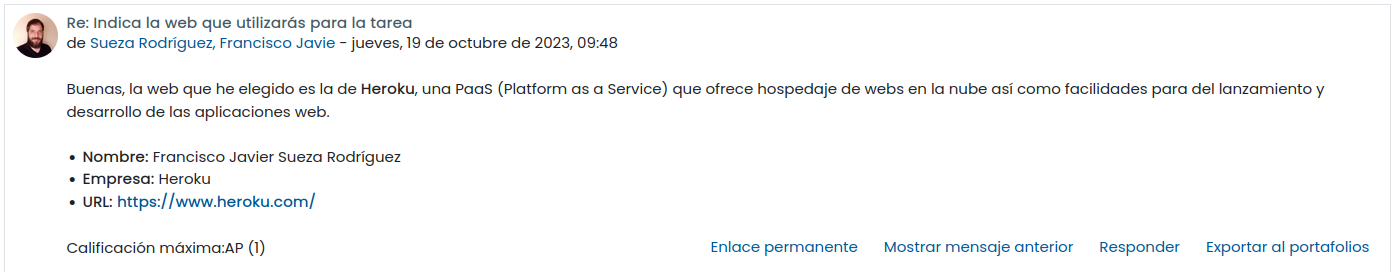
\includegraphics[scale=0.44]{aporte-foro.png}
    \caption{Aporte en el foro con la web seleccionada}
\end{figure}

Además de la página de Heroku, también he visitado la de \href{https://vercel.com/}{Vercel}, es otra \textbf{PaaS} (Platform as a Service) que ofrece servicios de hospedaje web y herramientas para el despliegue y desarrollo de aplicaciones web. A continuación se pueden ver dos capturas con las página principales tanto de Heroku como de Vercel.

\begin{figure}[H]
    \centering
    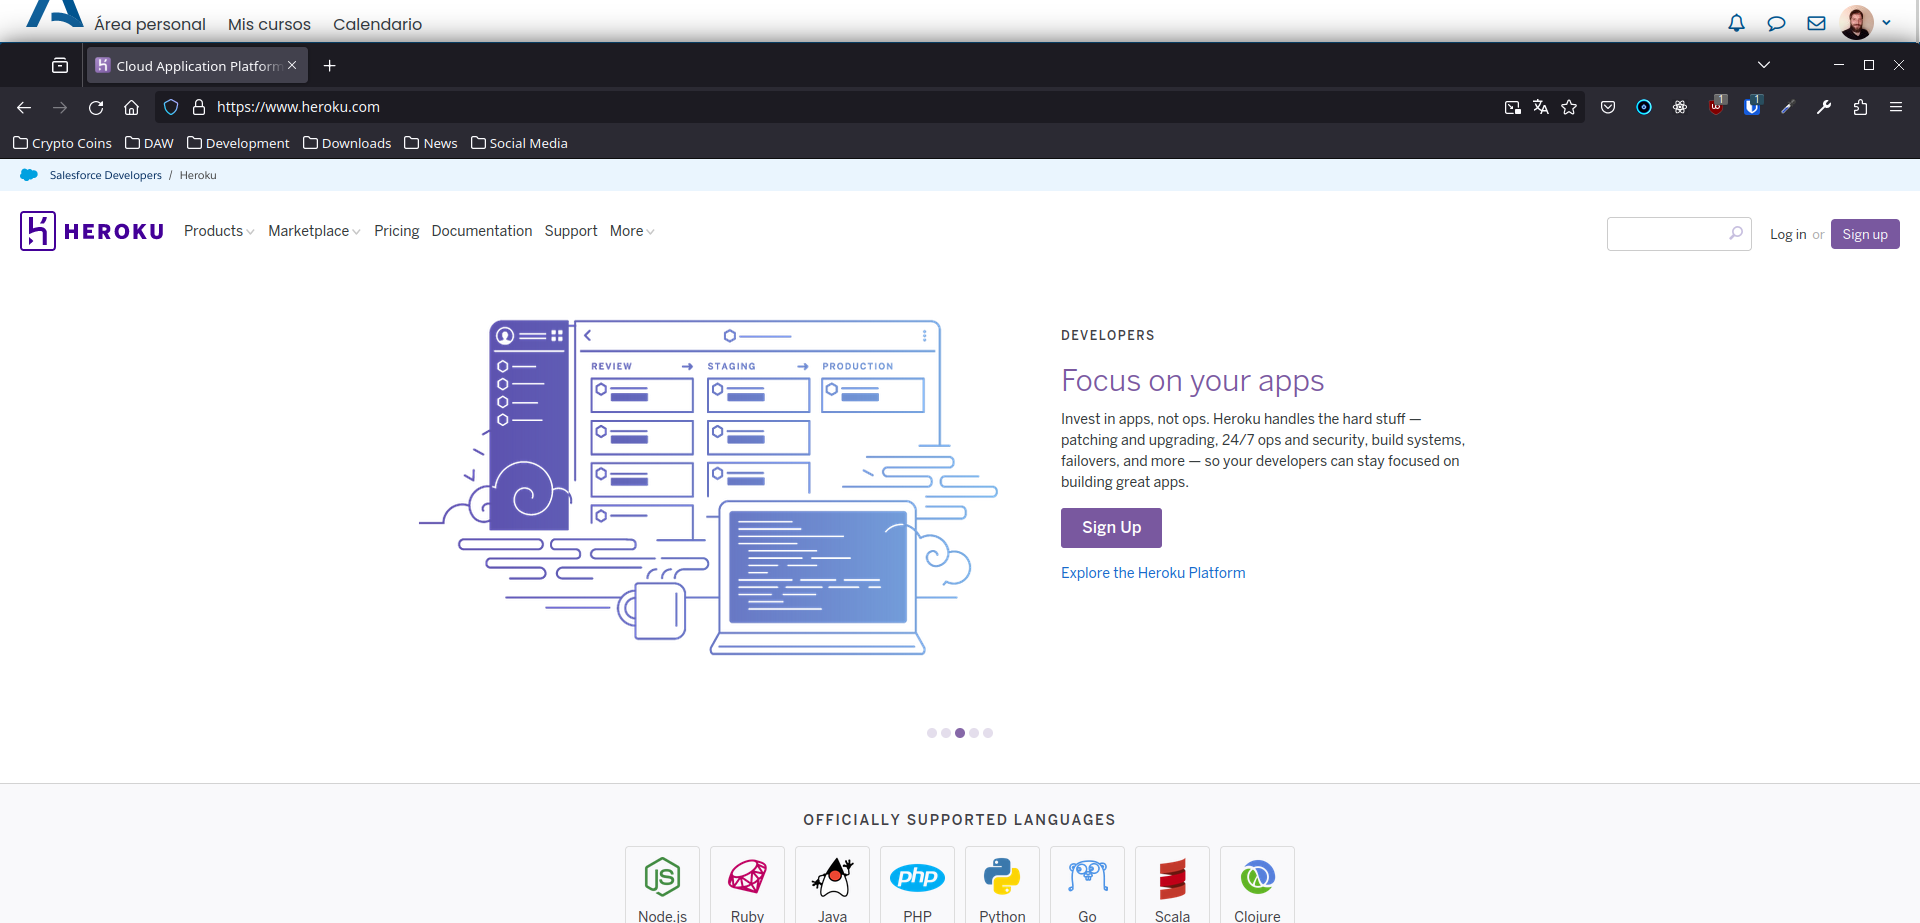
\includegraphics[scale=0.28]{heroku.png}
    \caption{Página principal de Heroku}
\end{figure}

\begin{figure}[H]
    \centering
    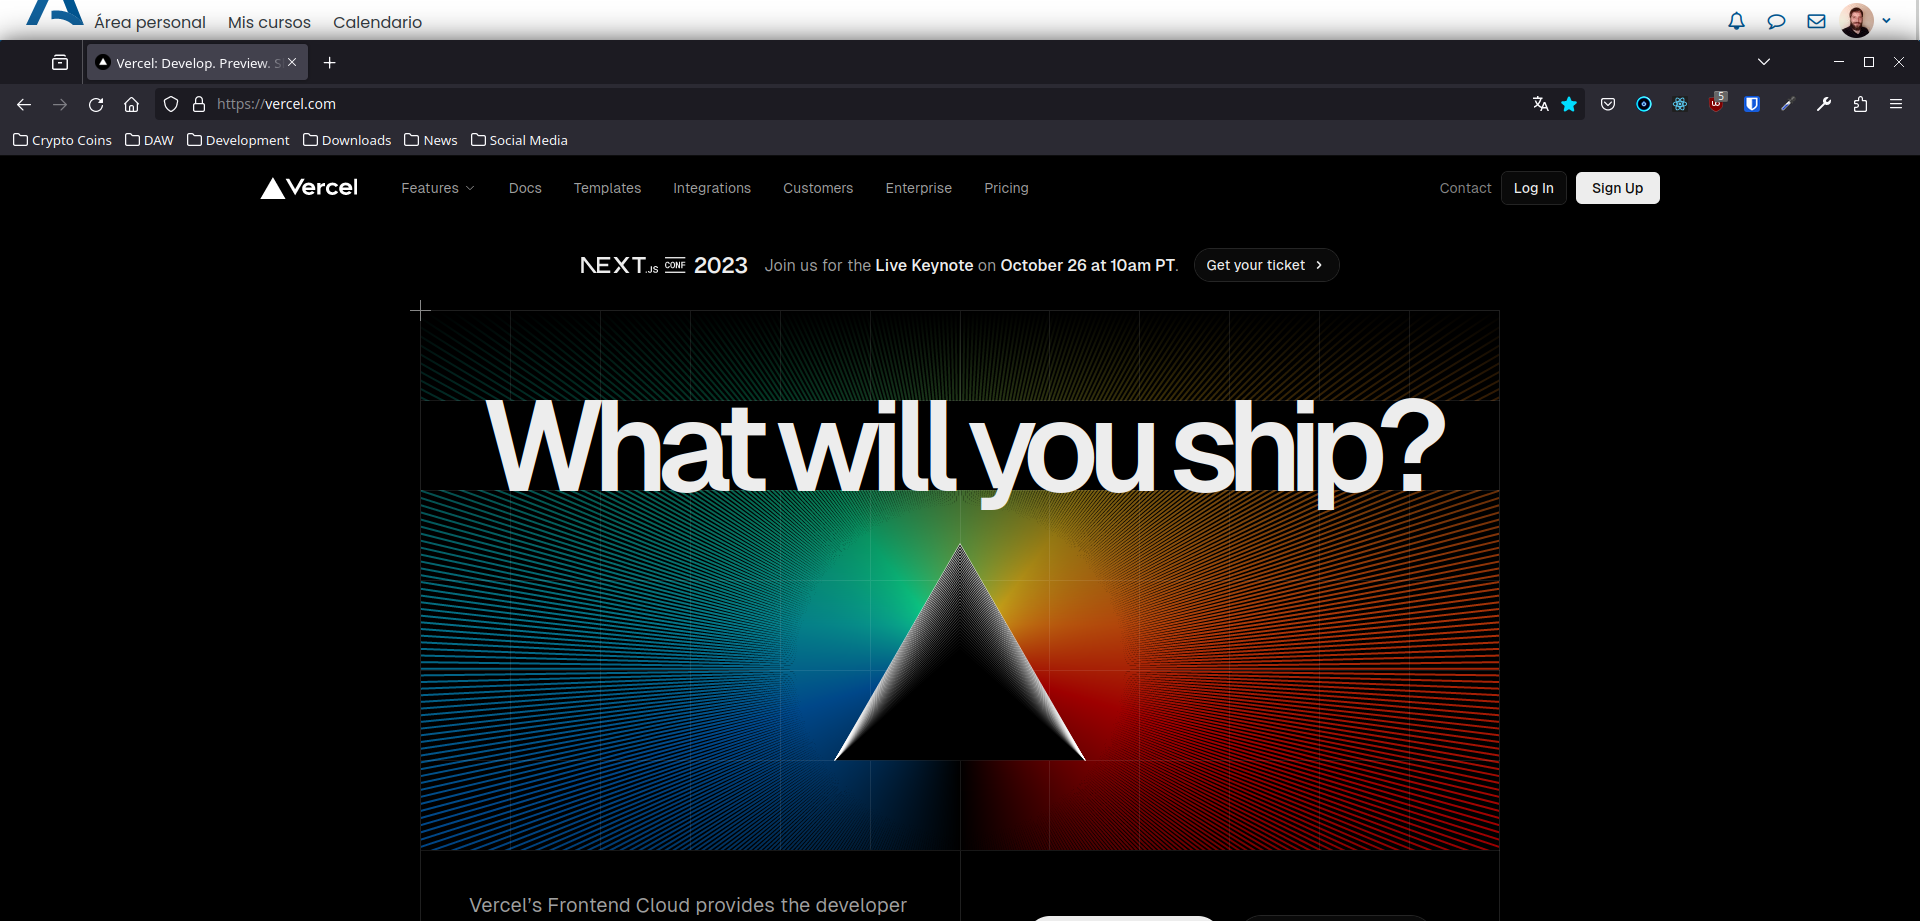
\includegraphics[scale=0.28]{vercel.png}
    \caption{Página principal de Vercel}
\end{figure}

Después de visitar las dos páginas, he decidido \textbf{elegir la de Heroku}. El \textbf{motivo} por el que se \textbf{ha elegido} esta es porque en la página web de Vercel \textbf{faltan elementos interactivos}, por lo menos en la página principal, que es la que vamos a analizar. Por lo que para efectos de esta tarea es más conveniente la selección de Heroku, ya que a la hora de analizarla vamos a poder realizar una análisis más completo.

A continuación, hemos \textbf{visualizado} la página web tanto en un \textbf{ordenador portátil}, con una pantalla de 15.4 pulgadas, como en un \textbf{dispositivo móvil}, con una pantalla de 5 pulgadas. En la siguiente figura podemos ver la capturas de la versión en sobremesa (parte izquierda de la imagen) y de la versión móvil (parte derecha).

\textbf{NOTA}: cabe señalar que debido a tamaño que tienen la capturas se han tenido que reducir para que quepan en la página, por lo que los detalles no se pueden apreciar todo lo bien que se debiera. Además, la captura en pantalla móvil se ha tenido que dividir por la mitad ya que sino era imposible que entrará en una página. Por esto, además de incluir las capturas en el documento, se van a adjuntar por si se quieren ver de forma más detallada.

\begin{figure}[H]
    \centering
    \fbox{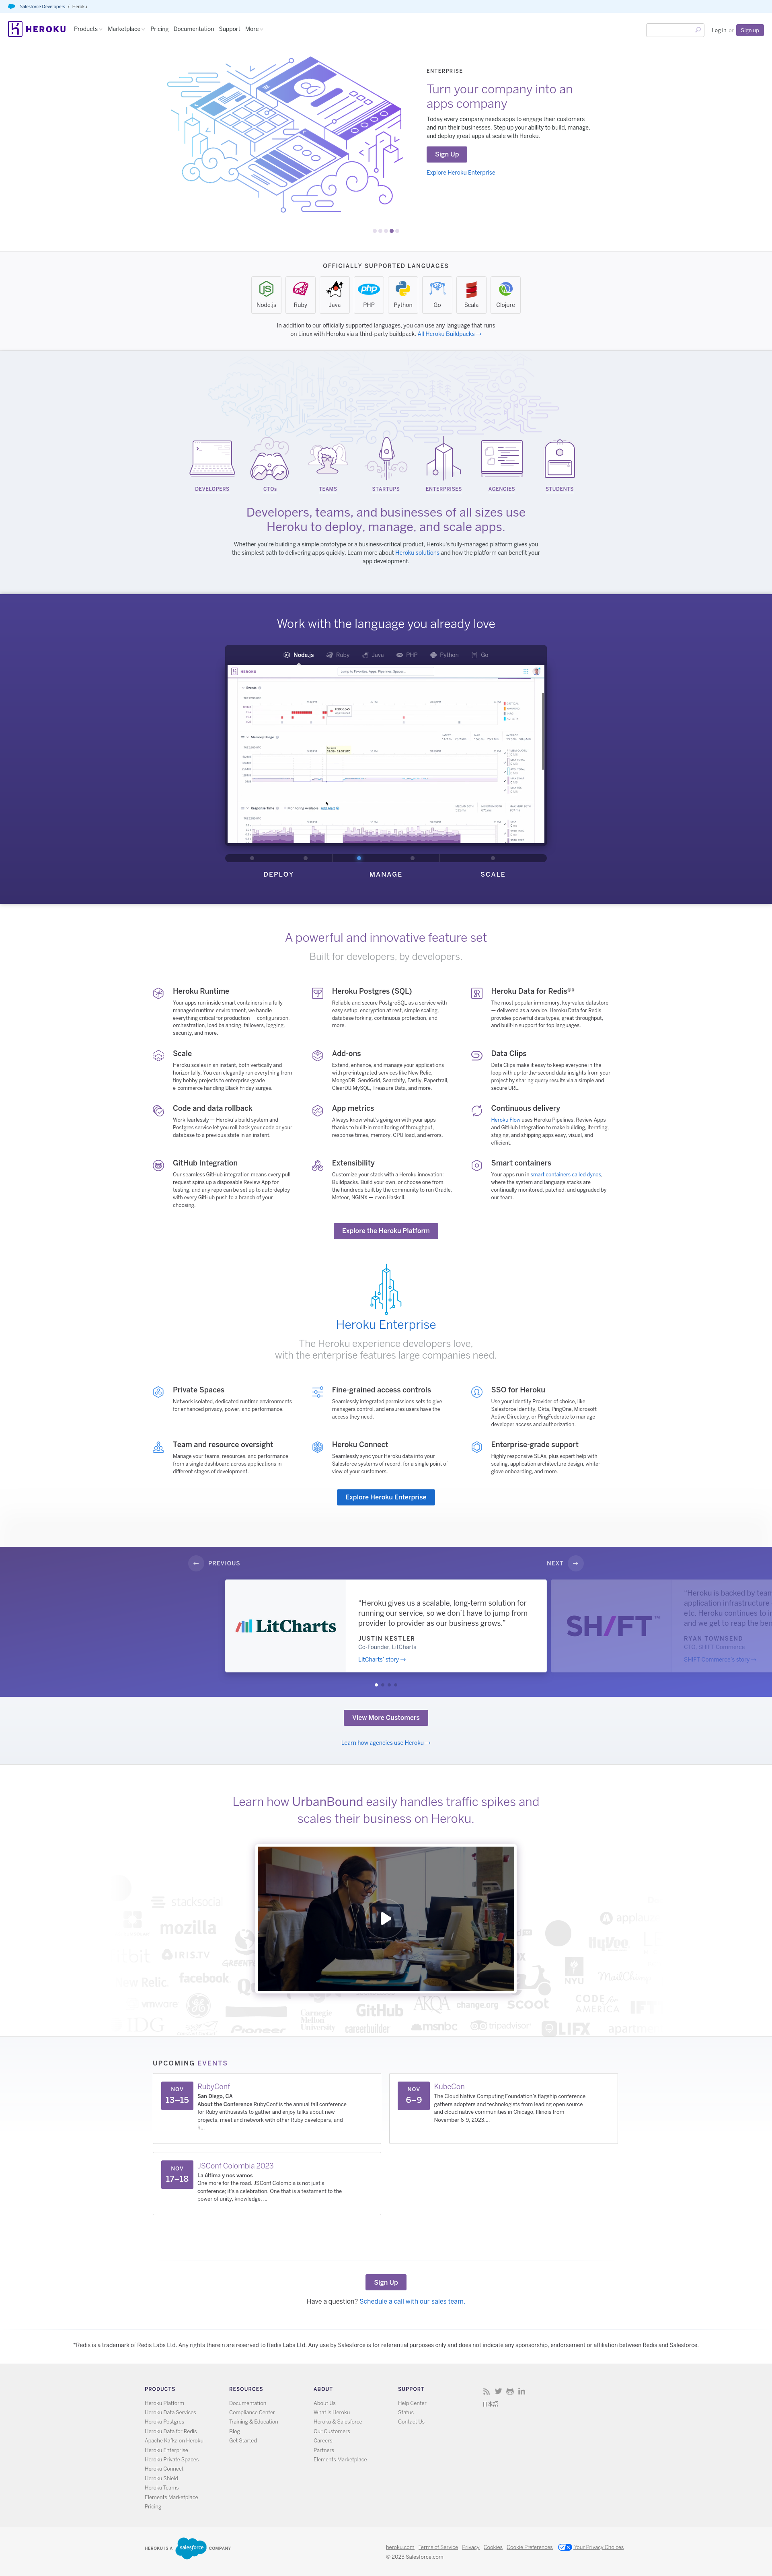
\includegraphics[scale=0.10]{heroku-completa-portatil.png}}
    \hspace{1cm}
    \fbox{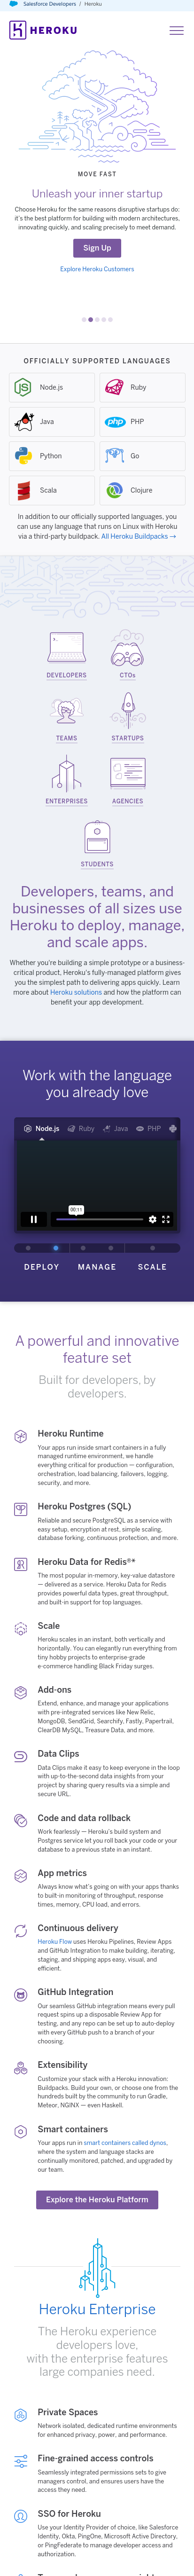
\includegraphics[scale=0.155]{heroku-completa-movil-1.png}}    \fbox{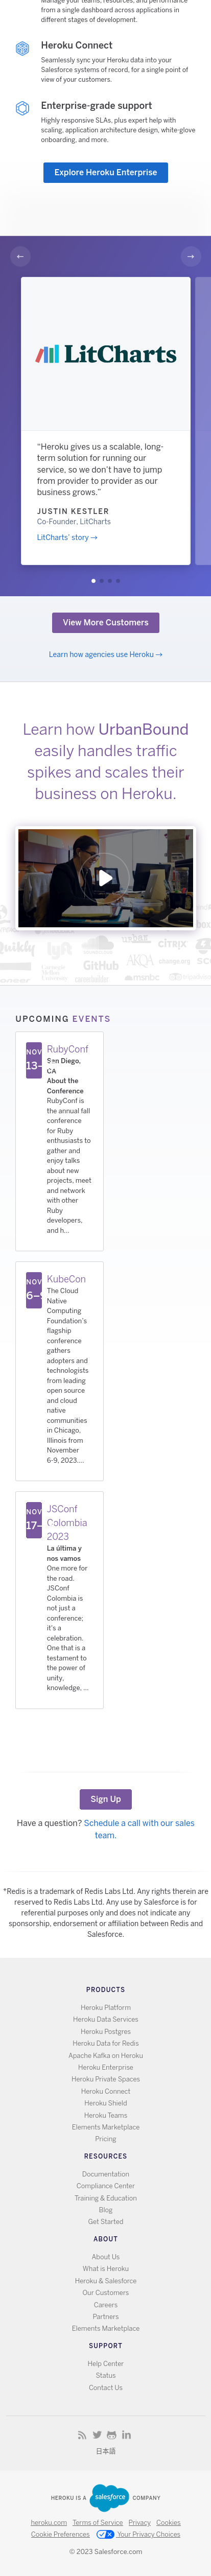
\includegraphics[scale=0.155]{heroku-completa-movil-2.png}}
    \caption{Página de Heroku en versión sobremesa (izquierda) y móvil (derecha)}
\end{figure}

Como podemos ver en las capturas anteriores, hay \textbf{significativas diferencias} entre la versión de ordenador y la versión móvil, 3 de estas diferencias son las siguientes:

\begin{itemize}
    \item \textbf{Menu de Navegación}: una de las diferencias más llamativas es el menú de navegación. Mientras que en la versión de ordenador se ha optado por \textbf{menú de navegación horizontal}, en la versión móvil tenemos un \textbf{menú hamburguesa}, para ahorrar espacio.

    \item \textbf{Alineación de los elementos}: otra de las diferencias principales es la alineación de los diferentes elementos como iconos, textos, etc. Mientras que en la versión de ordenador se aprovecha más el espacio horizontal y se usa más esta alineación, en la versión móvil se usa una alineación vertical, principalmente para que los elementos se puedan visualizar sin añadir scroll lateral a la página.

    \item \textbf{Formulario de Búsqueda}: en la versión para ordenador podemos ver algunos elementos interactivos en la parte superior derecha como un formulario de búsqueda, estos elementos desaparecen de la cabecera en la versión móvil y se integran, junto con el menú de navegación, en el menú hamburguesa.
\end{itemize}

\section{Ejercicio 2: Componentes de una Página Web}
\subsection{Enunciado}
Trabajando con la página web seleccionada y en la versión para ordenador, identifica y adjunta captura de pantalla de cada uno  de los componentes de la web:
\begin{itemize}
    \item \textbf{identificación}
    \item \textbf{navegación}
    \item \textbf{contenidos}
    \item \textbf{interacción}
\end{itemize}

\subsection{Solución}
En este ejercicio vamos a identificar varios componentes en la web de Heroku. Son las siguientes:

\begin{itemize}
    \item \textbf{Identificación}: la identificación la podemos encontrar en la parte superior izquierda de la página.

    \begin{figure}[H]
        \centering
        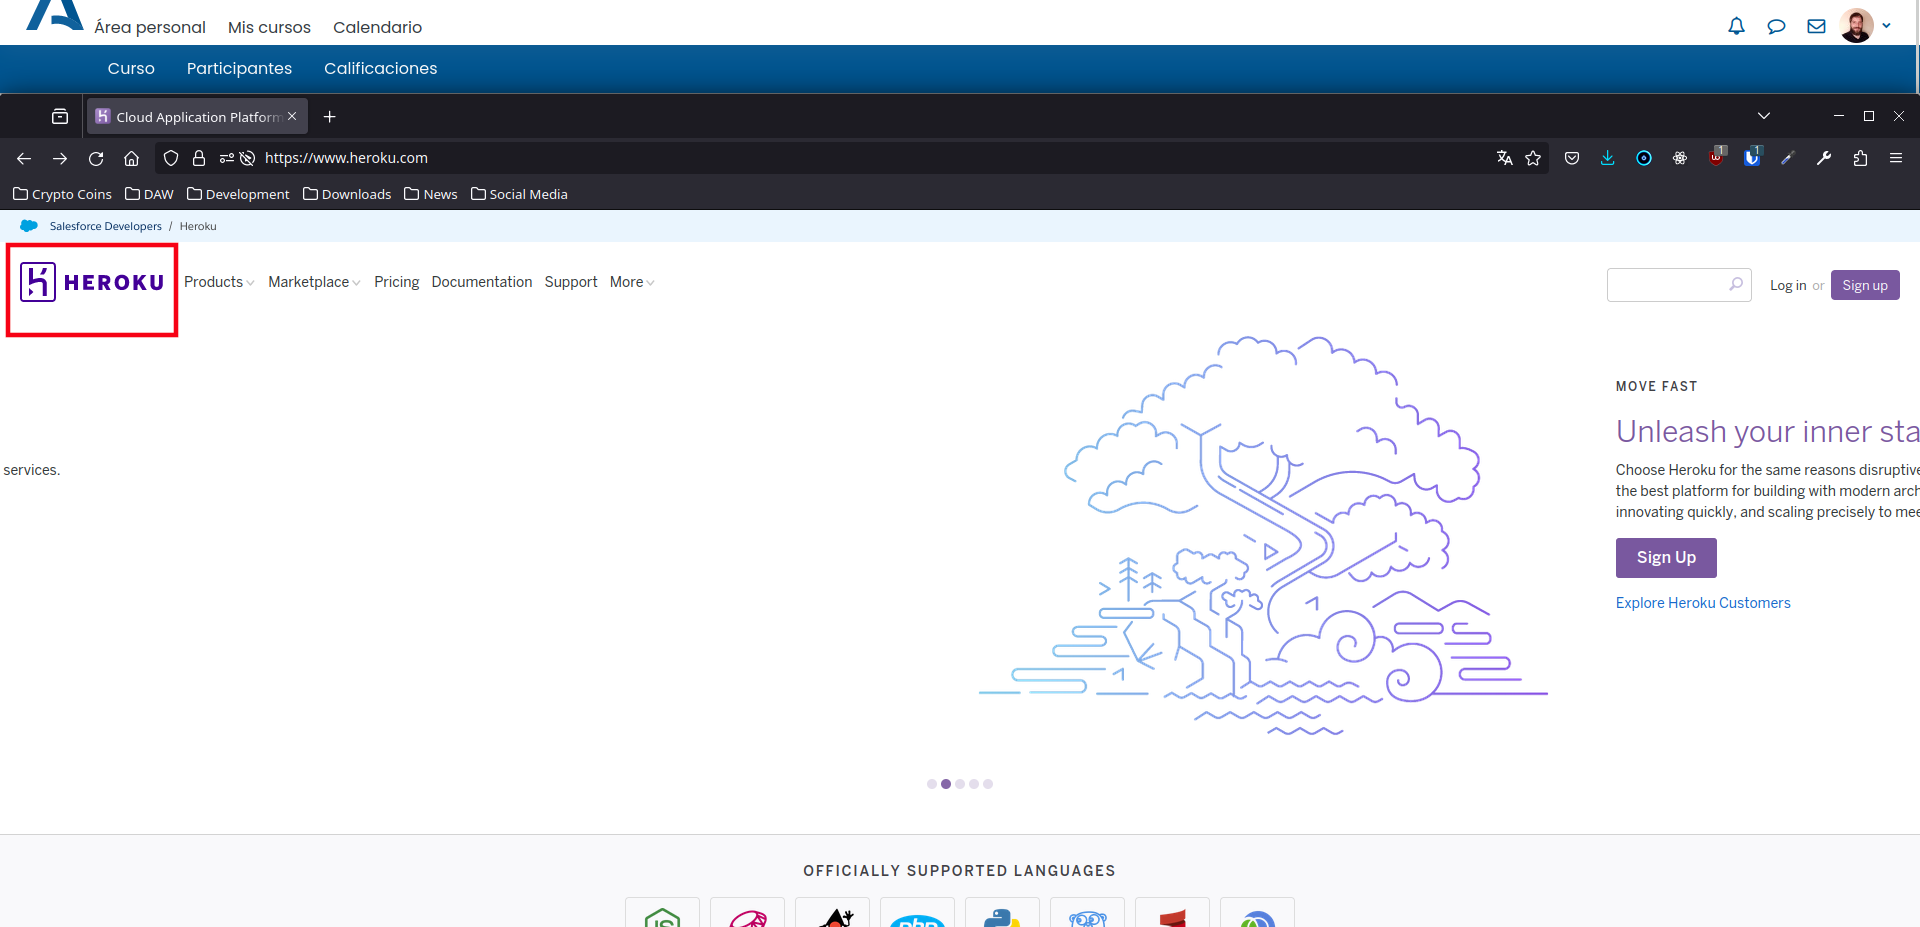
\includegraphics[scale=0.25]{heroku-identificacion.png}
        \caption{Identificación en la página de Heroku}
    \end{figure}

    \item \textbf{Navegación}: podemos encontrar dos zonas principales de navegación en la página principal de Heroku. Una se encuentra en la cabecera, a modo de menú de navegación horizontal, mientras que encima del pie de página, podemos encontrar otra zona de navegación con un menú de navegación vertical. Se han tomado dos capturas de ambas zonas de navegación.

    \begin{figure}[H]
        \centering
        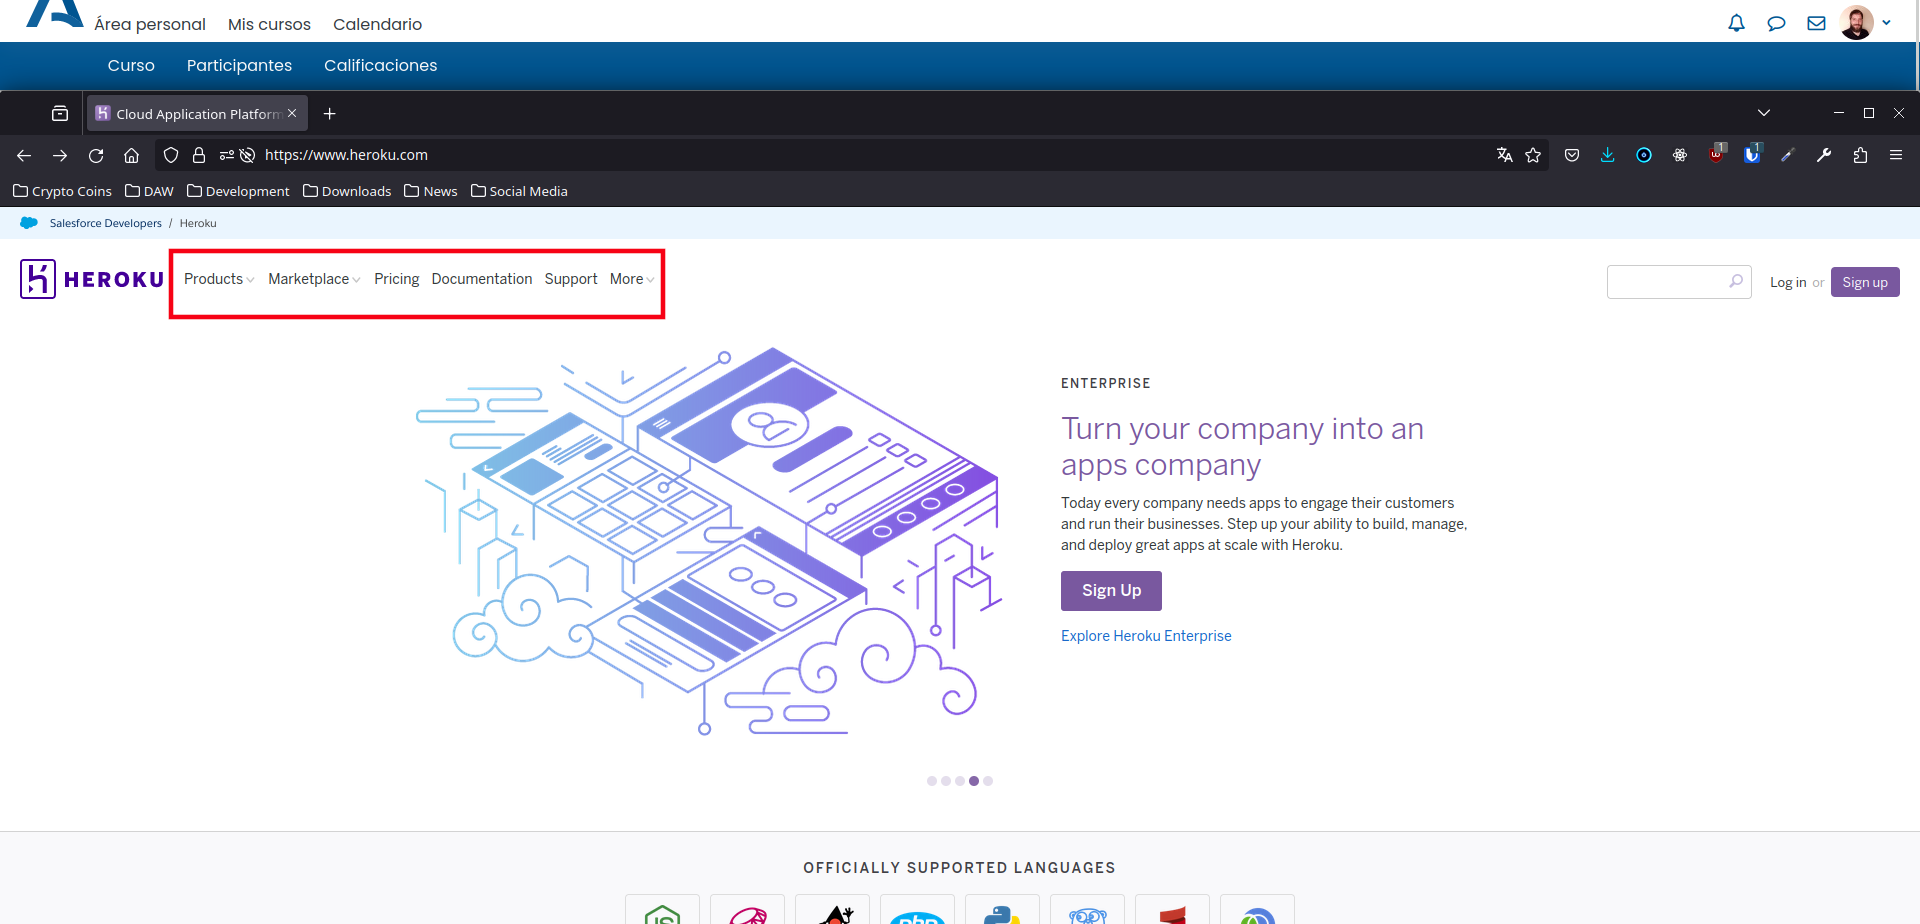
\includegraphics[scale=0.30]{heroku-navegacion-1.png}
        \caption{Zona de navegación superior de Heroku}
    \end{figure}

    \begin{figure}[H]
        \centering
        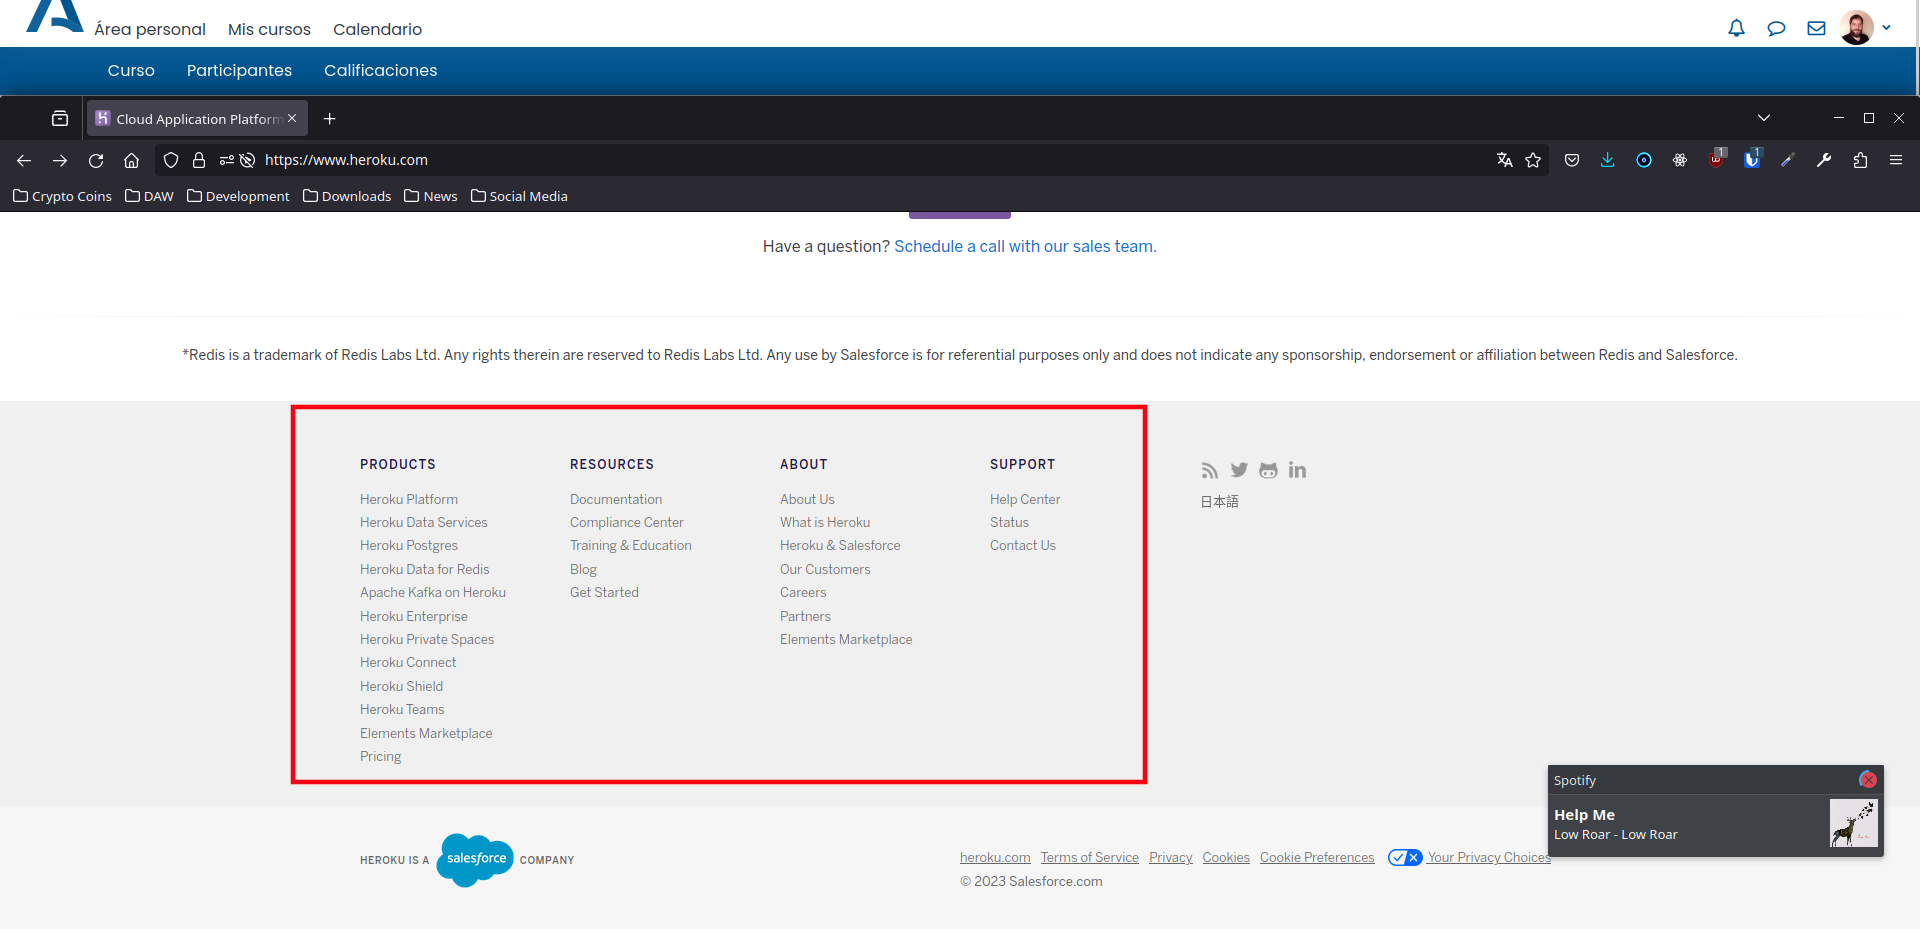
\includegraphics[scale=0.30]{heroku-navegacion-2.png}
        \caption{Zona de navegación inferior de Heroku}
    \end{figure}

    \item \textbf{Contenidos}: prácticamente el resto de la página, entre la cabecera y la zona de navegación interior esta destinada a contenidos, en concreto a exponer las herramientas y características del servicio.

    También hay una sección de \textbf{Upcoming Events}, donde aparecen los próximos eventos relacionados con la aplicación, como diferentes conferencias donde van a tener presencia. He elegido esta última parte como representativa de una zona de contenido, como se muestra en la siguiente figura.

    \begin{figure}[H]
        \centering
        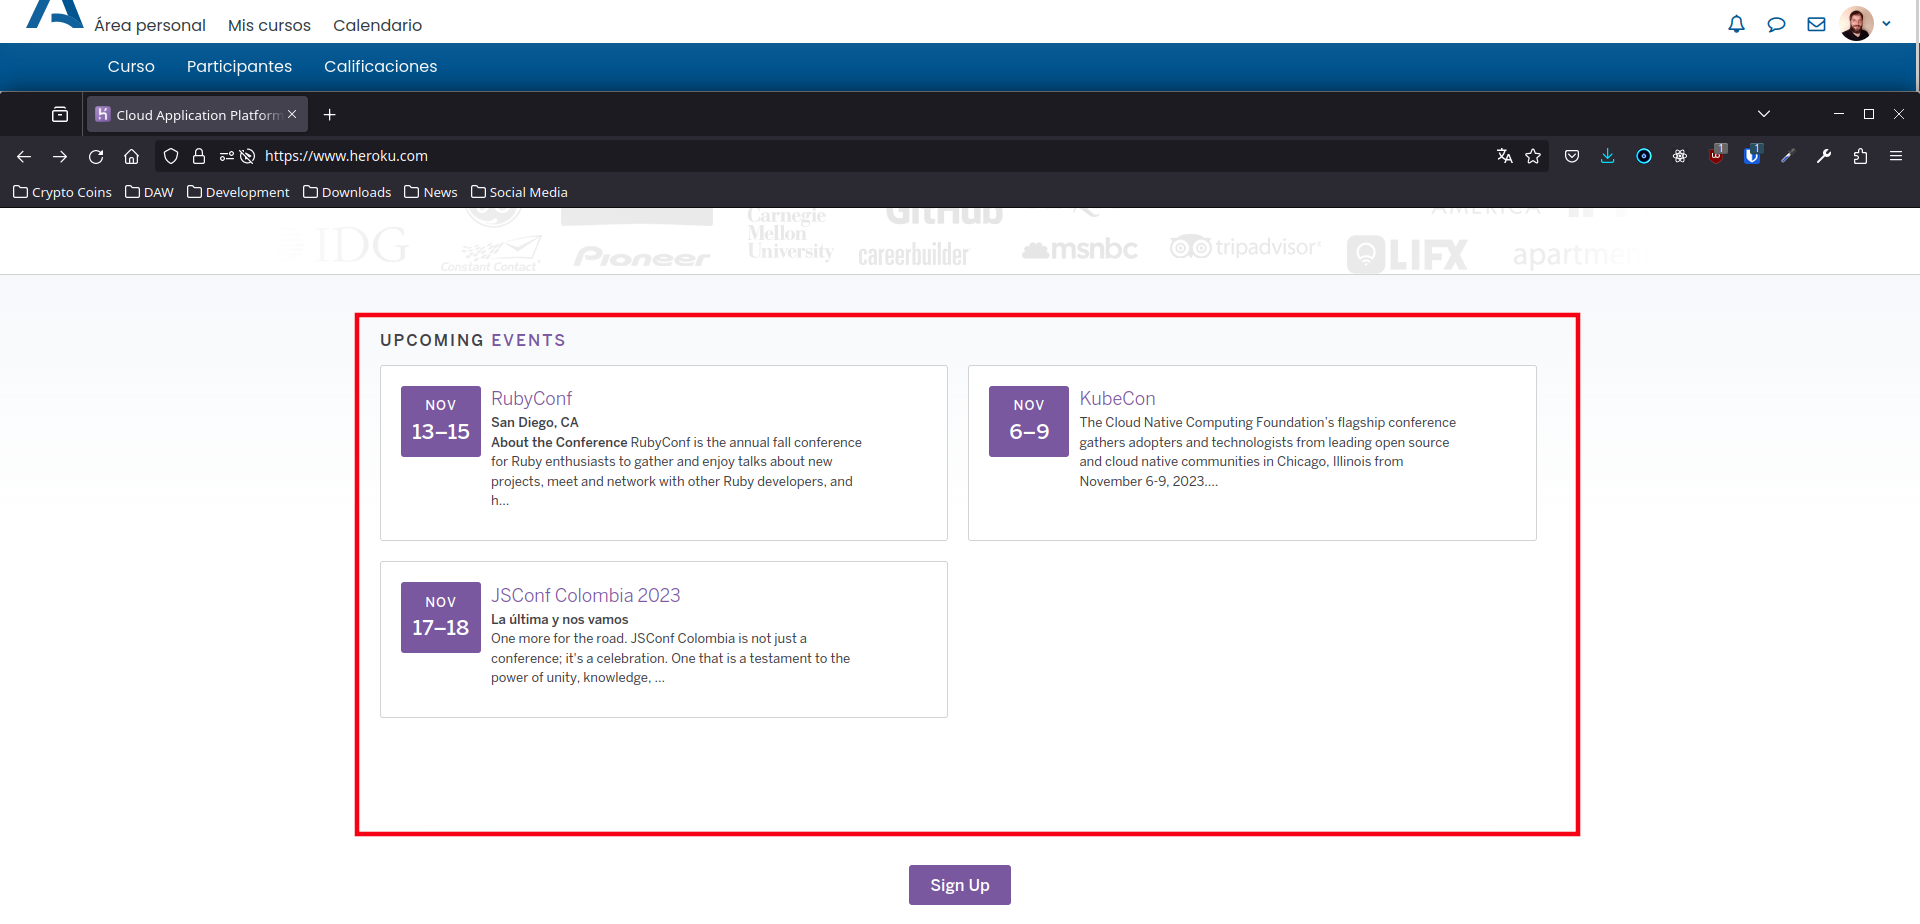
\includegraphics[scale=0.30]{heroku-contenido.png}
        \caption{Zona de contenido de Heroku}
    \end{figure}

    \item \textbf{Interacción}: la zona de interacción la podemos ver en la parte superior izquierda, donde hay un formulario donde podremos realizar búsquedas dentro de contenido de la web, como vemos en la siguiente imagen.

    \begin{figure}[H]
        \centering
        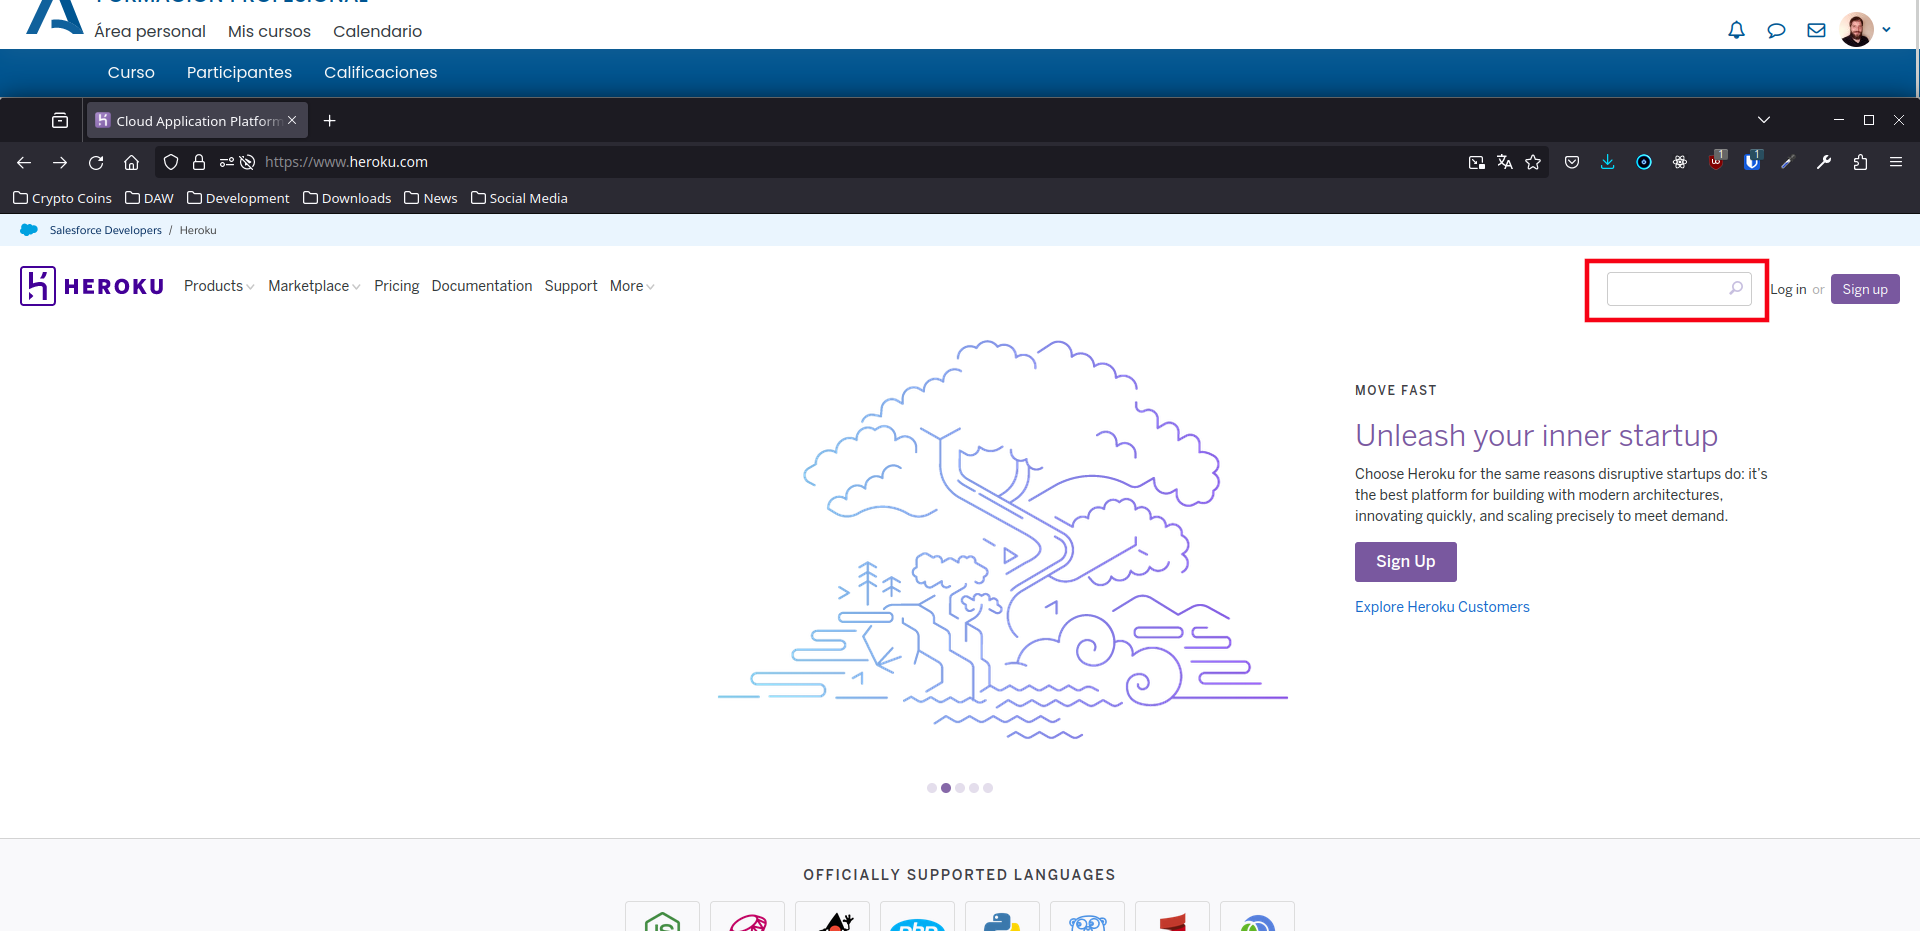
\includegraphics[scale=0.30]{heroku-interaccion.png}
        \caption{Zona de interacción de Heroku}
    \end{figure}
\end{itemize}

\section{Ejercicio 3: Principios de Gestalt}

\subsection{Enunciado}
Identifica dos principios de Gestalt de los que se citan en la unidad de trabajo, que se utilicen en la web seleccionada. En caso de que no encuentres ninguno, la web no será válida y tendrás que seleccionar otra. Para cada principio de Gestalt tendrás que:

\begin{itemize}
    \item indicar nombre del principio
    \item explicar en que consiste dicho principio.
    \item adjuntar captura de pantalla donde se pueda apreciar claramente el principio que estás indicando. Sobre la captura de pantalla puedes resaltar o marcar lo que consideres necesario para apreciar mejor el principio seleccionado. No debe darse nada por sobreentendido.
\end{itemize}

\subsection{Solución}
En la página web de Heroku podemos ver varios principios de Gestalt aplicados, aunque nosotros nos vamos a centrar en los dos siguientes:

\begin{itemize}
    \item \textbf{Principio de Proximidad}: este principio se basa en el hecho de que la mente suele agrupar los elementos en función de las distancia que hay entre ellos. En la página de Heroku, en concreto en el menú de navegación inferior, podemos ver como a pesar de que todos los enlaces son iguales, nuestra mente los agrupa según su proximidad, no viéndolos como una amalgama de enlaces, sino como 4 listas de enlaces bien diferenciadas, como vemos a continuación.

    \begin{figure}[H]
        \centering
        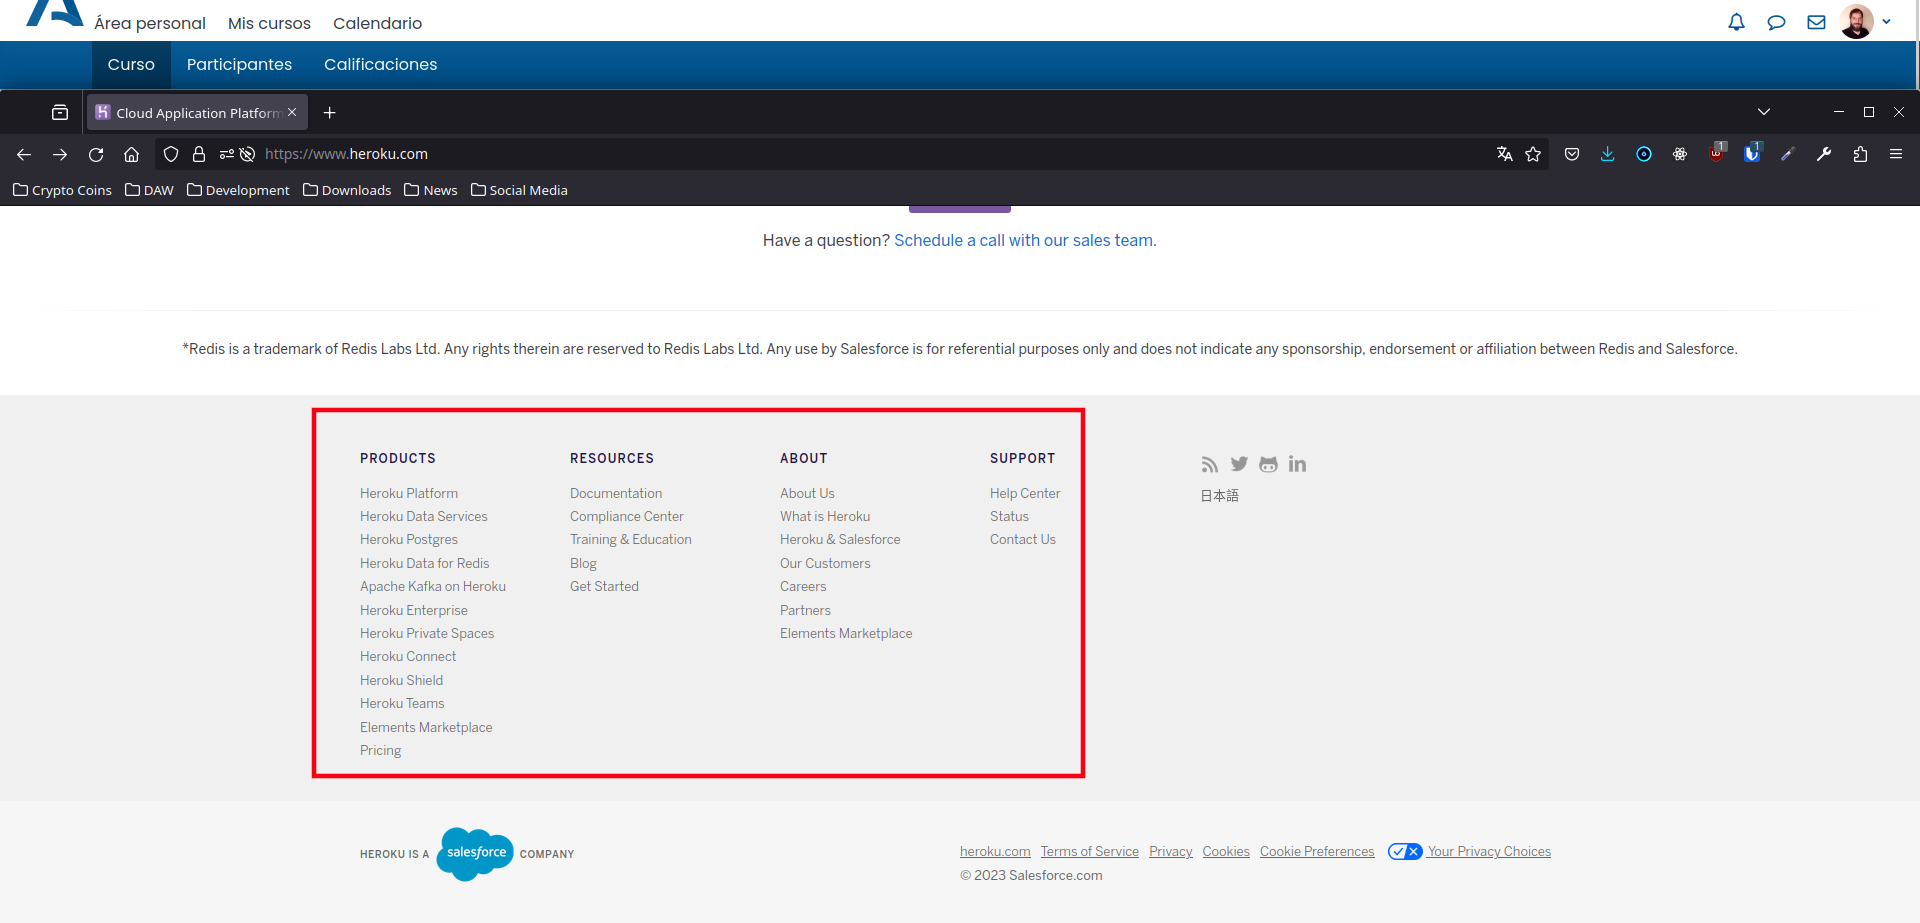
\includegraphics[scale=0.24]{heroku-gestalt-2.png}
    \end{figure}

    \item \textbf{Principio de Continuidad}: este principio establece que nuestra mente suele percibir los elementos continuos, aunque su contorno este interrumpido. En las ilustraciones que podemos ver en la parte superior de la página, vemos como se aplica este principio. En el ejemplo de la imagen de abajo podemos ver un árbol, montañas o nubes, aunque ninguna de sus formas esta completamente cerrada.

    \begin{figure}[H]
        \centering
        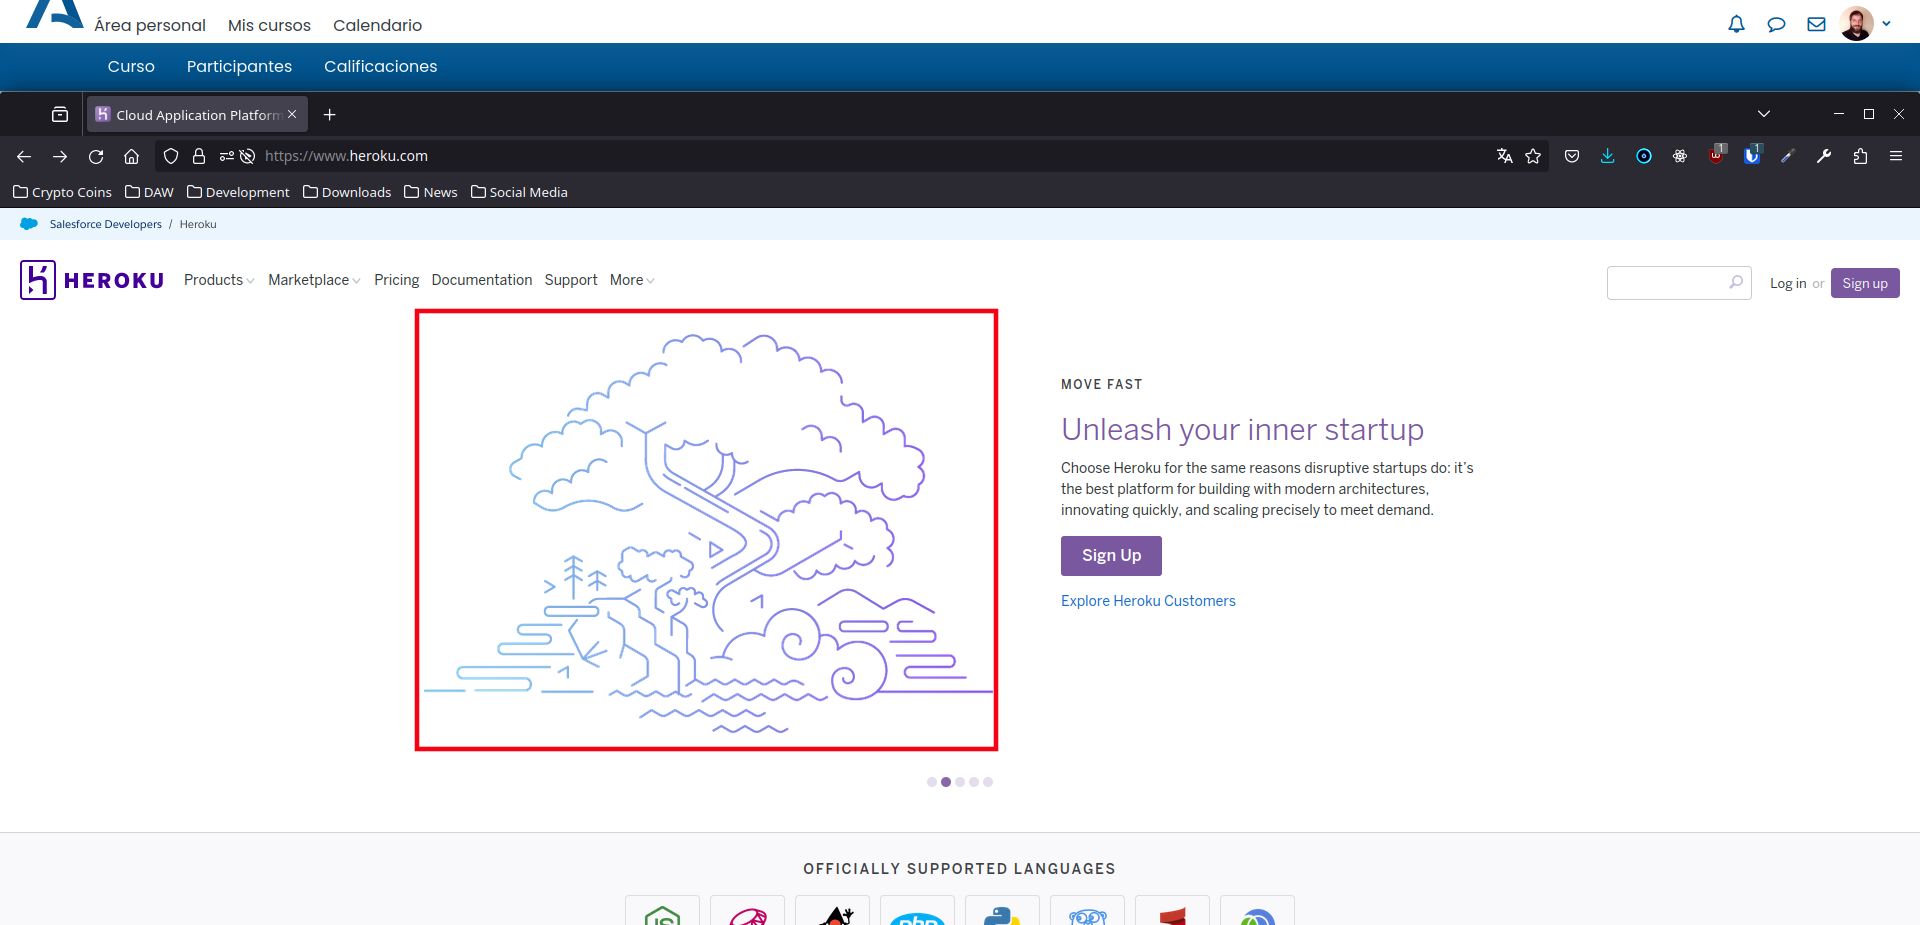
\includegraphics[scale=0.24]{heroku-gestalt-1.png}
    \end{figure}
\end{itemize}

\section{Ejercicio 4: Guía de Estilo}

\begin{enumerate}[label=\alph*)]
    \item Define que es una guía de estilo.
    \item Da tres razones por lo que es bueno trabajar con una guía de estilo.
    \item Busca una guía de estilo en internet, adjúntala y comente brevemente que te parece el documento. Indica la URL de donde la has obtenido o descargado o se puede visitar.
    \item Vamos a analizar los elementos más importantes que componen una guía de estilo, para ello nos centraremos en la web que has seleccionado en el ejercicio 1 (y que como se ha indicado debe ser única para cada alumno y alumna).
    \begin{itemize}
        \item Reconoce el logotipo de la Web. (adjunta captura de pantalla).
        \item Reconoce dos recursos gráficos que tengan funcionalidades (o finalidades) y naturaleza (imágenes, iconos, etc..) diferentes dentro de la página principal que estás analizando. Indica para cada tipo de recurso cual es su finalidad o funcionalidad (adjunta una captura de pantalla por cada recurso). Si los recursos son de igual naturaleza o funcionalidad solo se valorará uno.
        \item Analiza el menú (estructura o sistema) de navegación de la versión de escritorio. Adjunta captura de pantalla y comenta al menos:
        \begin{itemize}
            \item Dos virtudes.
            \item Un defecto que encuentres.
            \item Las respuestas tienen que estar justificadas de forma razonada.
        \end{itemize}

        \item Indica el tipo de estructura (prototipos) del mapa de navegación que utiliza la web. En caso de que no exista mapa de navegación en la web seleccionada, busca un mapa de navegación en otra web e indica la estructura que tiene. Debes adjuntar URL, captura de pantalla e indicar y justificar el tipo de mapa de navegación que utiliza.

        \item Reconoce una tipografía que se utilice en la web, indica para la fuente seleccionada:
        \begin{itemize}
            \item Para qué se utiliza.
            \item Captura de pantalla donde se vea dónde se utiliza.
            \item Captura de pantalla donde se vea el nombre de la fuente. Para ello puedes valerte del modo desarrollador del navegador o alguna extensión o plugin.
        \end{itemize}

        \item Analiza la paleta de colores que utiliza la página seleccionada (al menos dos colores diferentes). Debes indicar para cada color:
        \begin{itemize}
            \item Qué elementos la utilizan, debes adjuntar captura de pantalla donde se vea claramente la zona del color a la que haces referencia.
            \item Código de color en RGB, debes valerte de una herramienta, extensión (como colorZilla) o modo desarrollador, donde se vea claramente la zona de la pantalla a la que haces referencia y el código RGB. No vale con poner solo el código del color o mostrar la zona, deben verse a la vez color y código.
            \item Indica qué se persigue en la interfaz con ese color y qué te transmite. Puedes consultar la parte de la unidad relacionada con la psicología del color para dar respuesta a esta pregunta.
        \end{itemize}
    \end{itemize}
\end{enumerate}

\subsection{Solución}
En este ejercicio vamos a responder varias preguntas sobre las guías de estilo y ha identificar sus elementos en la página que hemos seleccionado.

\begin{enumerate}[label=\alph*)]
    \item Una \textbf{Guía de Estilo} es un conjunto de normas y reglas para el diseño de una página web. En ella se estipulan elementos como el tamaño y posicionamiento de imágenes, los tipos de fuentes y el tamaño que tendrán estás dependiendo de su funcionalidad, la paleta de colores que se va a emplear, los iconos e imágenes, el posicionamiento de los elementos en los diferentes bloques de la página web, etc...

    \item El uso de guías de diseño tiene muchas \textbf{ventajas}, entre las que caben destacar las siguientes:
    \begin{enumerate}
        \item \textbf{Ahorro de Tiempo}: el uso de guías de diseño nos va a ahorrar tiempo en el proceso de diseño de una Web, ya que muchas de las decisiones que debemos tomar vienen ya indicadas en la guía, sin tener nosotros que pensar en, por ejemplo, que tipo de fuente vamos a usar para los encabezados o la paleta de colores a elegir. Todo eso viene ya definido en la guía.

        \item \textbf{Uniformidad}: el empleo de la guía ayuda a que todas las páginas Web que pertenecen al sitio tengan el mismo estilo, lo que hace que el sitio Web se vea más consistente y sea más agradable navegar por él.

        \item \textbf{Mantenimiento}: el uso de la guía de estilo hace que el mantenimiento de la aplicación sea más simple y rápido de realizar, ahorrando tiempo y dinero.
    \end{enumerate}

    \item La guía seleccionada ha sido la \textbf{Guía de Estilo y Manual de Buenas Prácticas para} de la \textbf{Universidad de Granada}, para el diseño de sitios web institucionales de la UGR.

    Está guía me parece muy completa ya que no solo trata los aspectos gráficos de las web corporativas de la UGR, sino que también trata aspecto como la accesibilidad, que es algo bastante importante en el desarrollo Web. Se definen además como se deben emplear diferentes elementos como los encabezados, los colores, etc.., además de desaconsejar el uso de diferentes tecnologías como los frames. En general, me parece una guía \textbf{bastante completa}.

    \item En este punto vamos a \textbf{identificar} los elementos más importantes de una guía en las página web seleccionar, en nuestro caso, la de Heroku. Los elementos, aparecen resaltados con una cuadrado de color rojo.

    \begin{itemize}
        \item \textbf{Logotipo de la Web}: se encuentra en la parte superior izquierda de la cabecera.

        \begin{figure}[H]
            \centering
            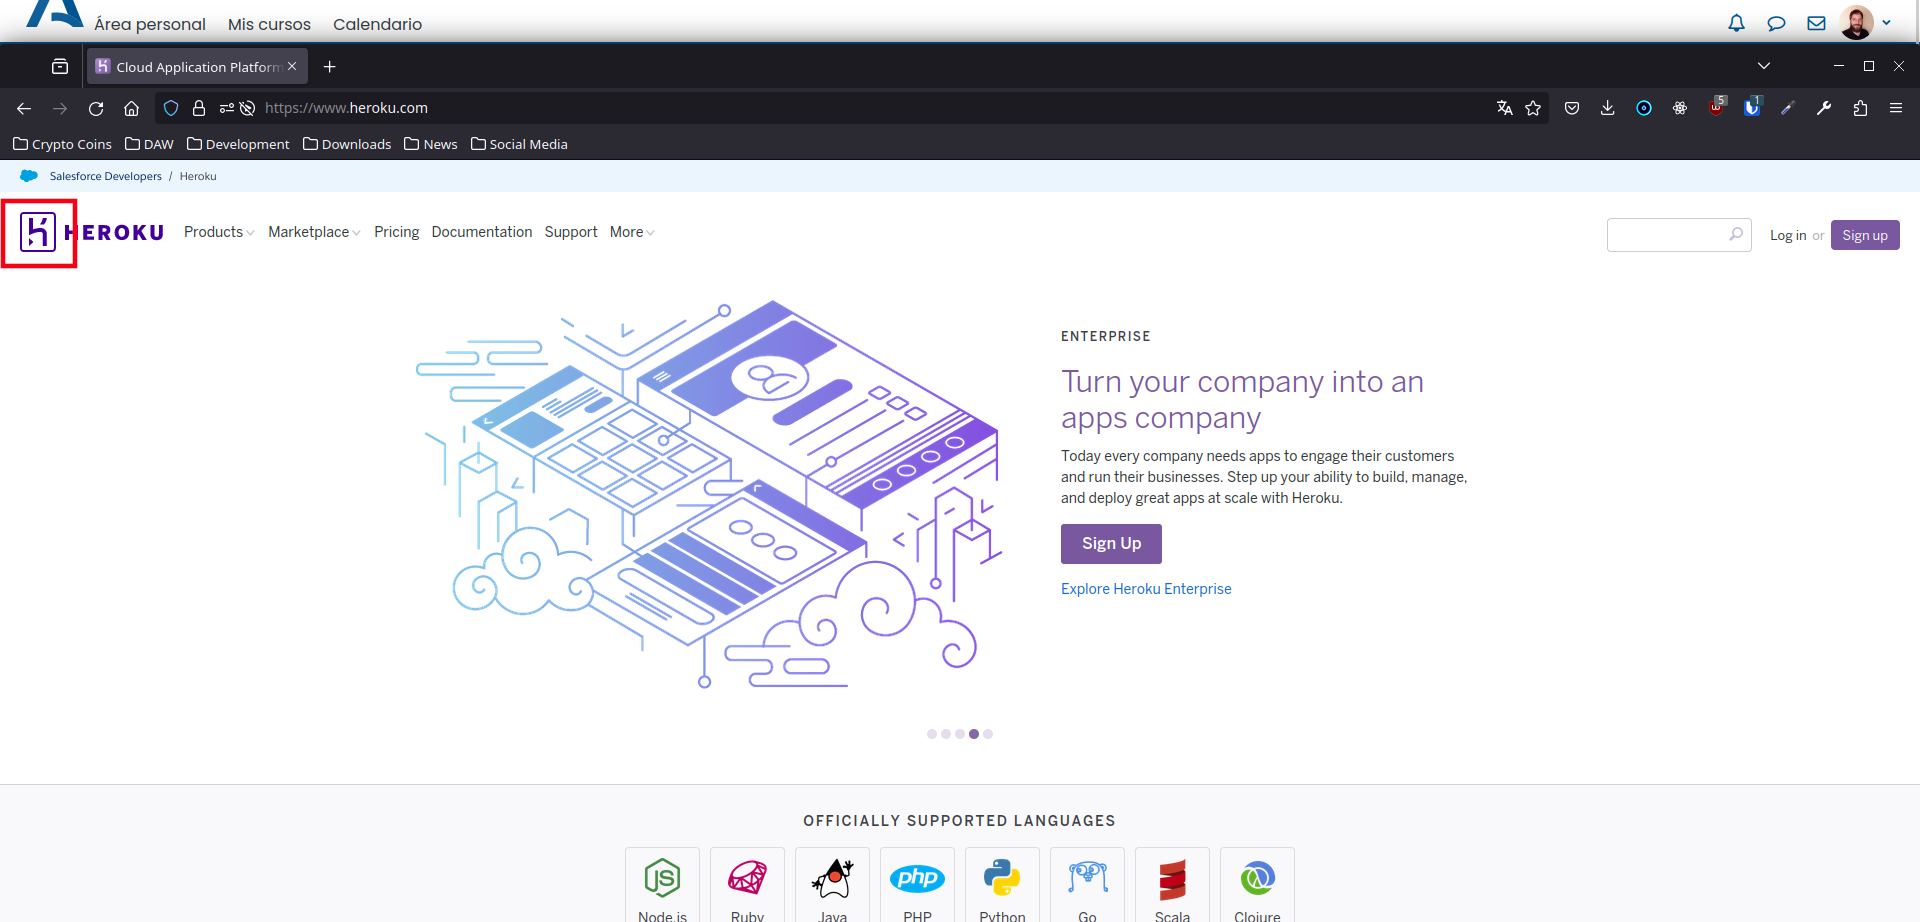
\includegraphics[scale=0.28]{heroku-logo.png}
        \end{figure}

        \item Se han identificado dos elementos con gráficos con funcionalidades diferentes, estos son:
        \begin{itemize}
            \item \textbf{Ilustración de Cabecera}: en la cabecera tenemos diferentes ilustraciones que aparecen junto a textos, describiendo algunas de las características de la plataforma. Estas ilustraciones tiene una \textbf{función meramente decorativa}.

            \begin{figure}[H]
                \centering
                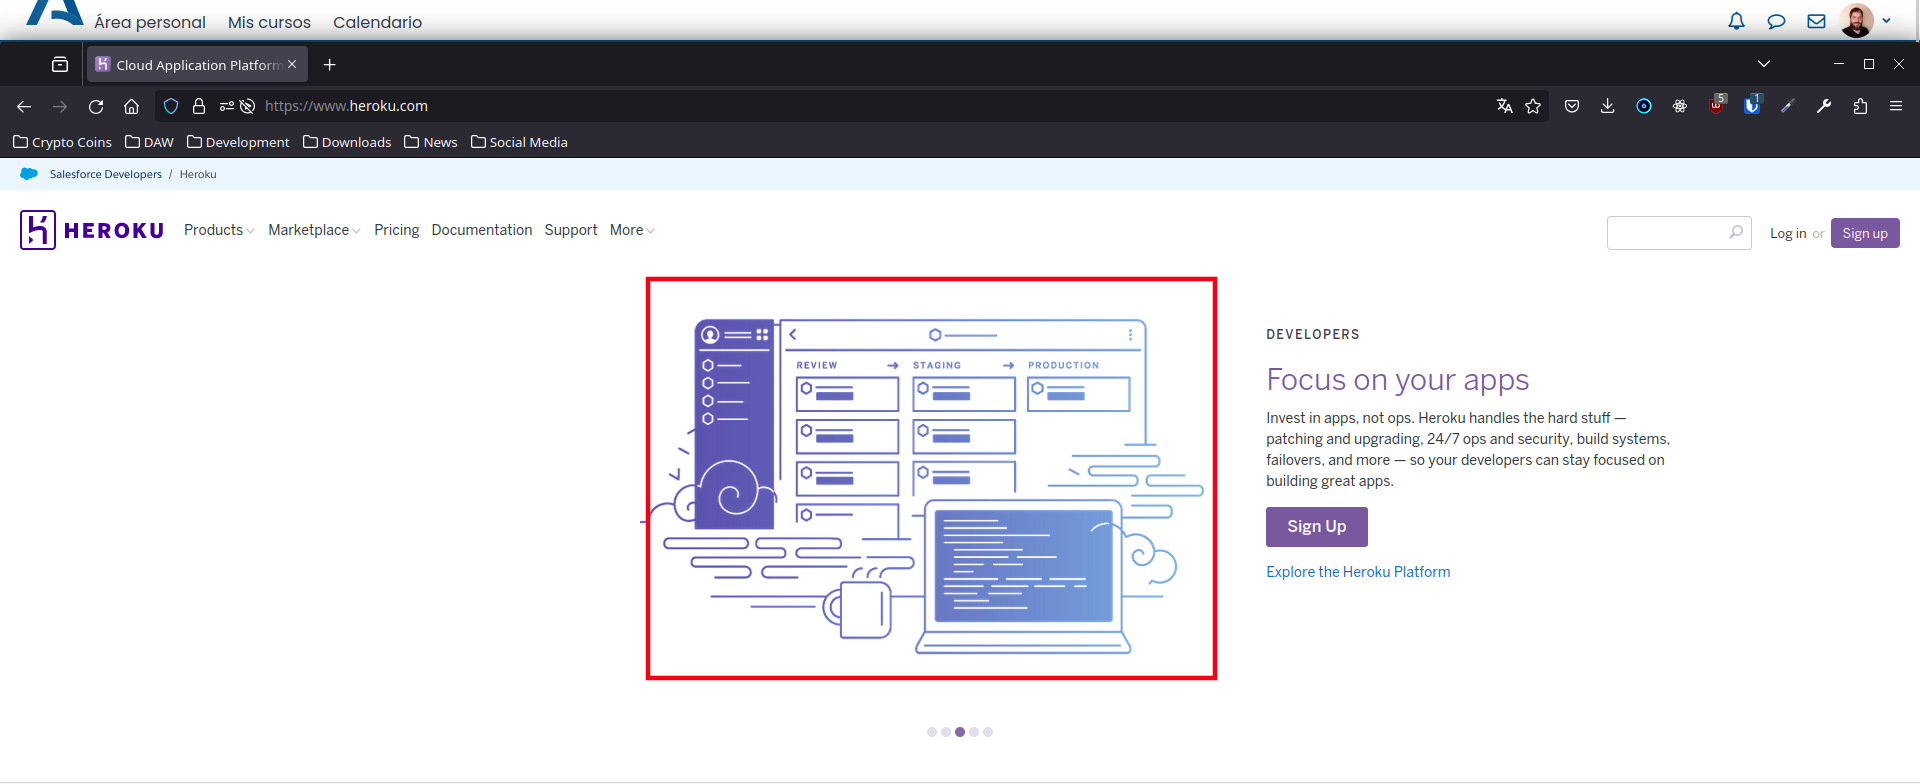
\includegraphics[scale=0.28]{heroku-grafico-1.png}
            \end{figure}

            \item \textbf{Iconos de Tecnologías}: el segundo elementos son los iconos que acompañan a las diferentes tecnologías que soporta la plataforma. En este caso, la \textbf{función} de estos iconos es la de \textbf{identificar a las marcas que representan}.

            \begin{figure}[H]
                \centering
                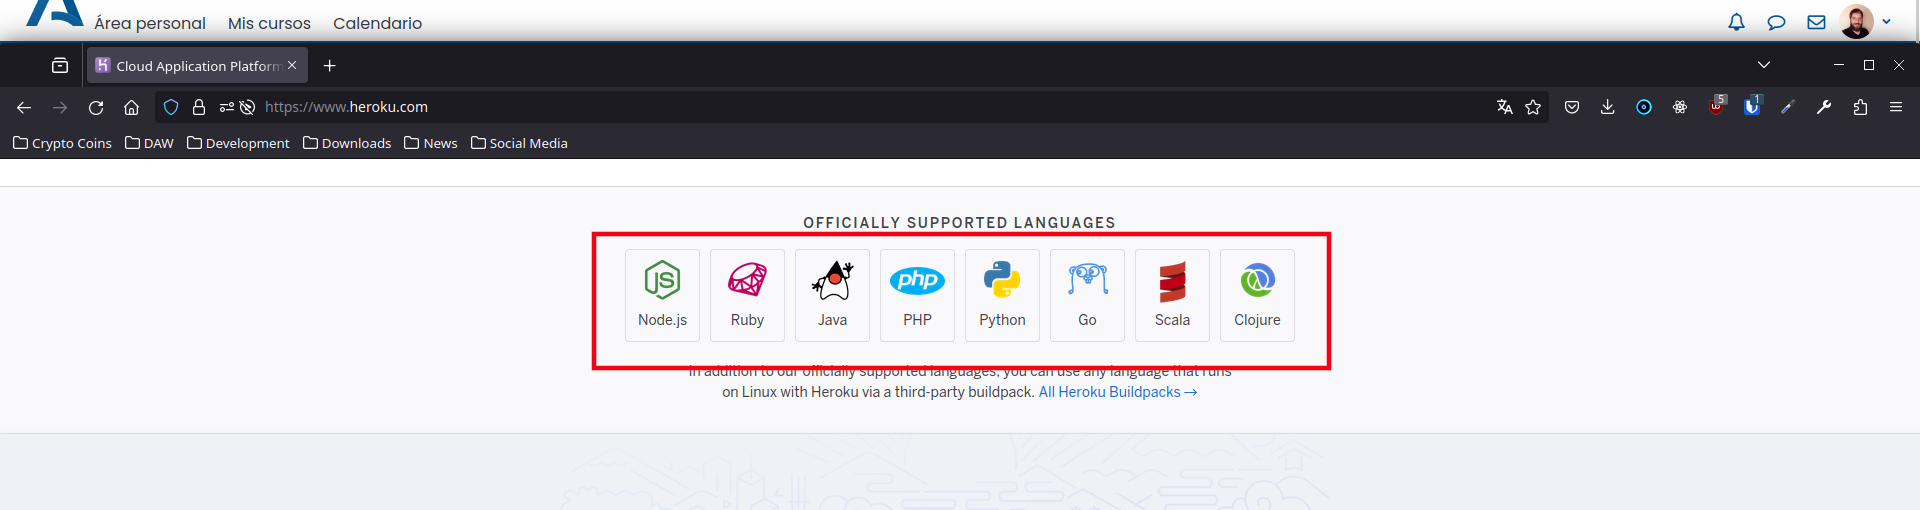
\includegraphics[scale=0.28]{heroku-grafico-2.png}
            \end{figure}
        \end{itemize}

        \item El siguiente punto que vamos a analizar es el \textbf{menú} de Heroku, en su versión de escritorio, que podemos ver en la siguiente captura.

        \begin{figure}[H]
            \centering
            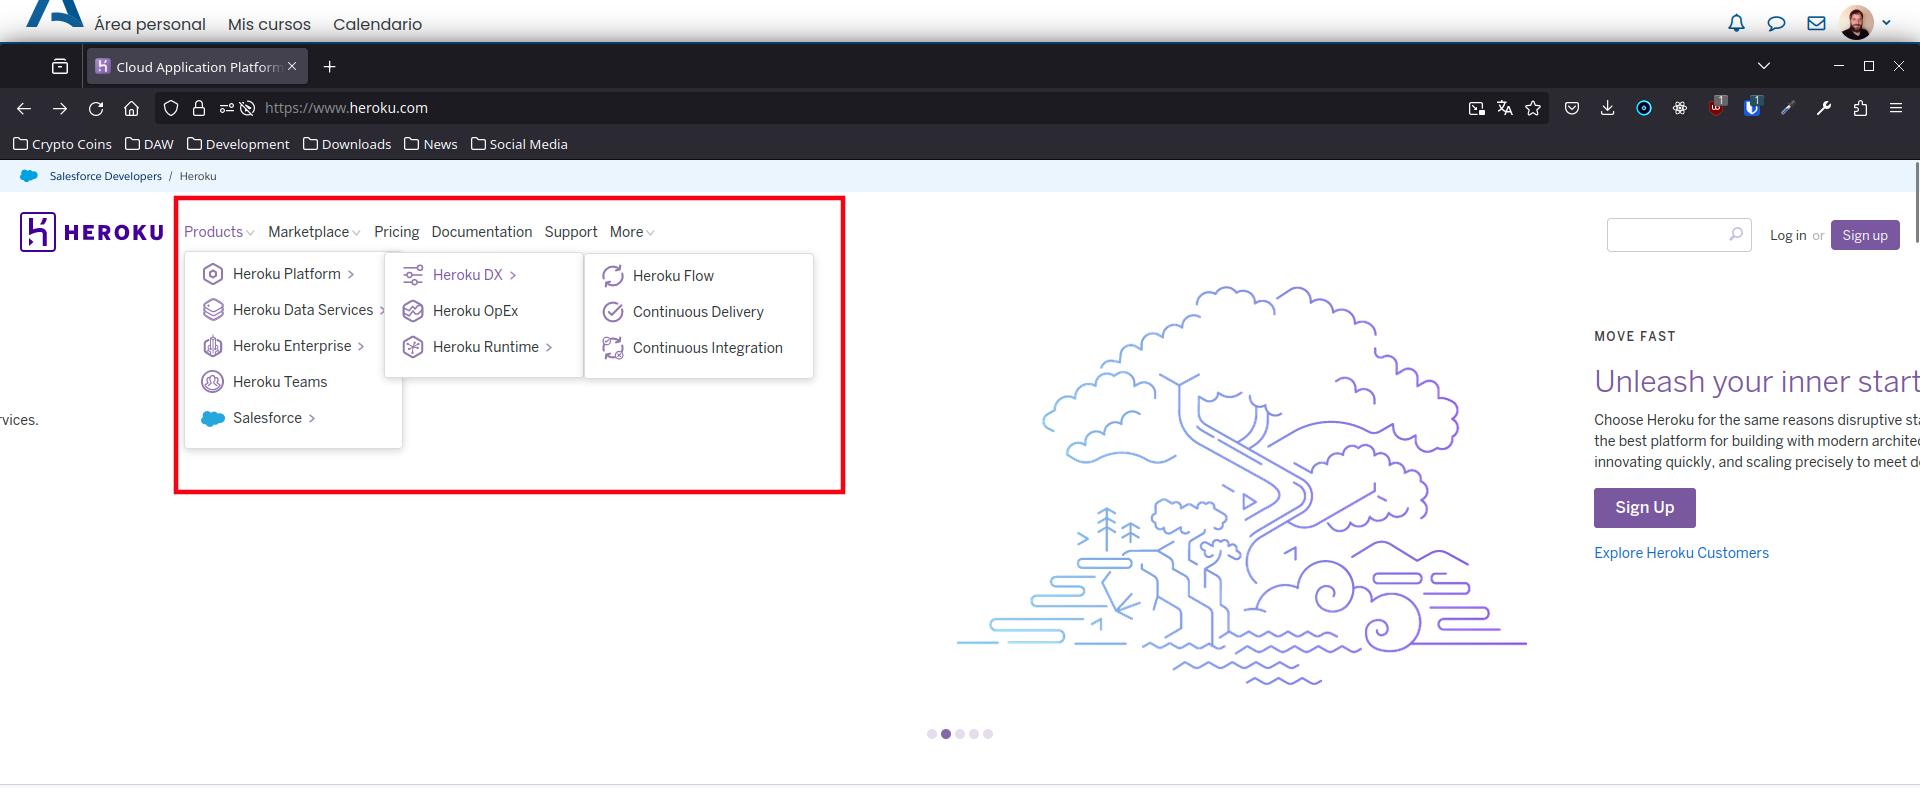
\includegraphics[scale=0.28]{heroku-menu.png}
        \end{figure}

        El menú esta bastante bien elaborado, si hubiera que destacar \textbf{2 virtudes} serían:
        \begin{itemize}
            \item \textbf{Organización}: es una menú bastante limpio y bien organizado, que hace encontrar cualquier elemento sea sencillo.
            \item \textbf{Elegante}: es un menú bonito, visualmente, y los iconos le añaden un elemento gráfico que resalta este aspecto.
        \end{itemize}

        Aunque el menú esta muy bien a nivel general, si hay \textbf{un defecto} que podríamos destacar:
        \begin{itemize}
            \item \textbf{Accesibilidad}: el menú ademas de tener una letra pequeña, aunque eso puede que también dependa de como esta configurado mi ordenador, carece de elementos de accesibilidad, sería, por ejemplo, adecuado incluir texto alternativo a los enlaces del menú, que puedan ser leídos por un screen reader.
        \end{itemize}

        \item Respecto al \textbf{mapa del sitio}, Heroku no tiene un mapa del sitio como tal, por lo que hemos elegido el \textbf{mapa} de la \textbf{web de la Universidad de Granada}, que podemos ver en la siguiente captura.

        \begin{figure}[H]
            \centering
            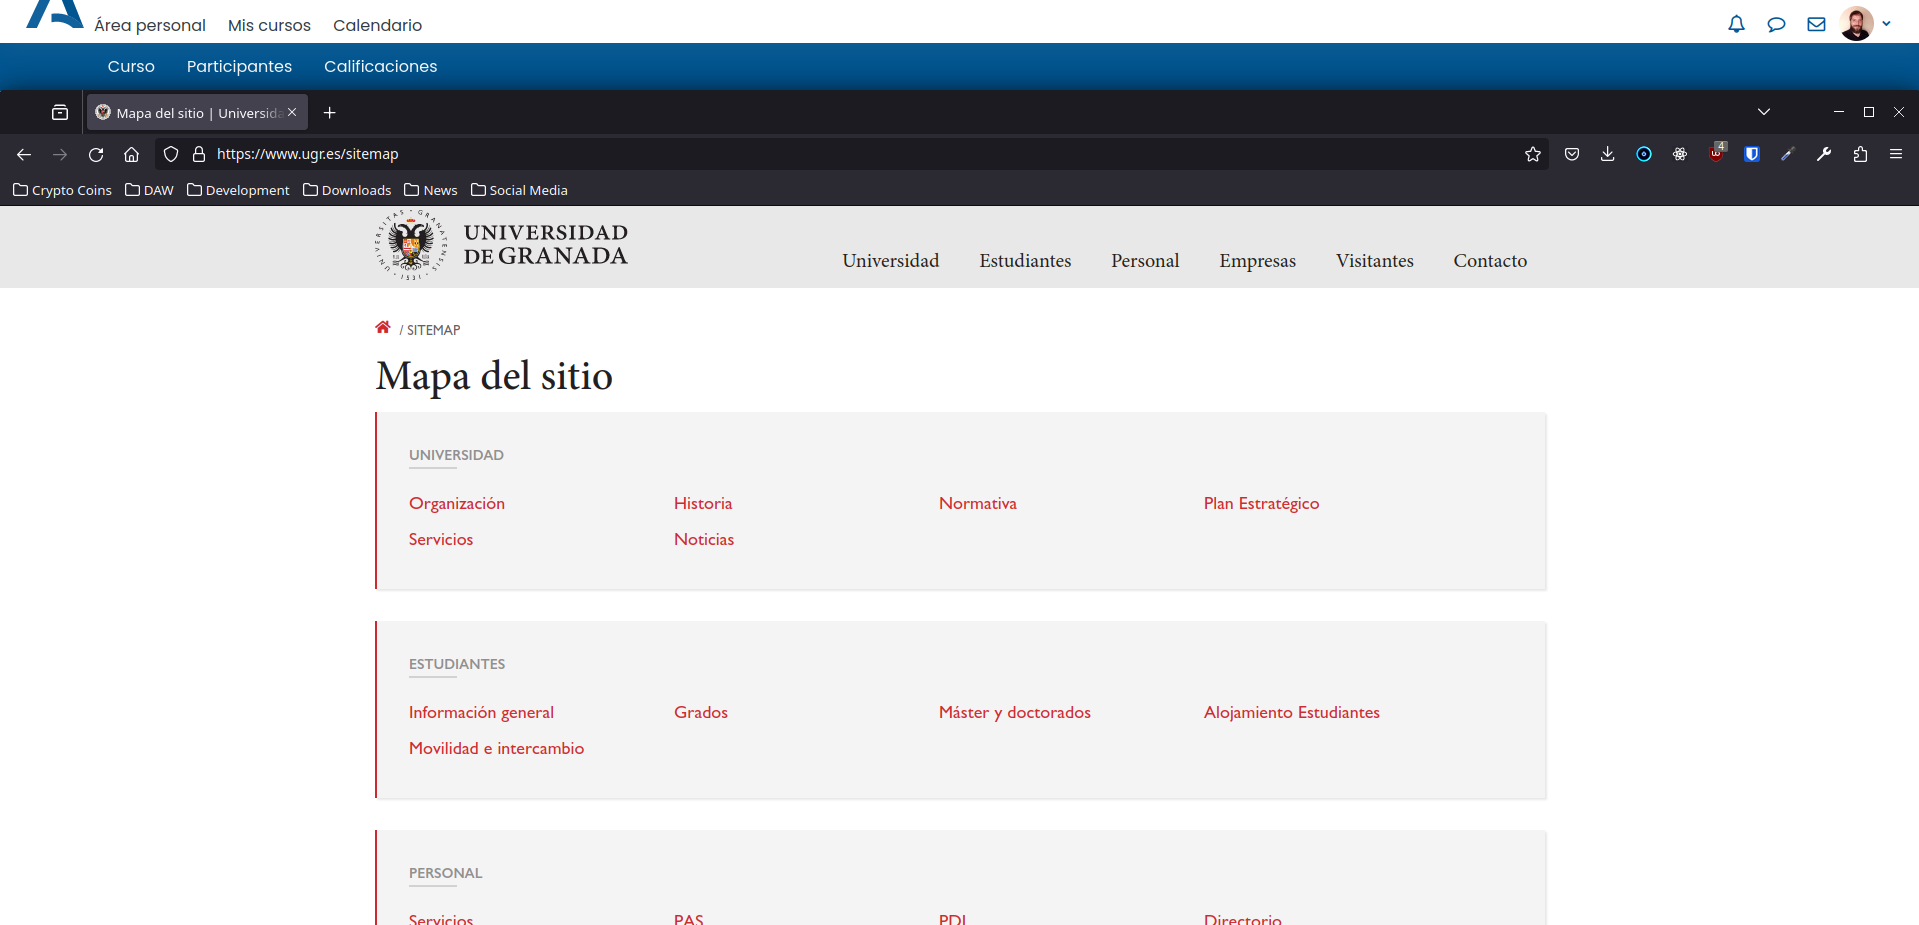
\includegraphics[scale=0.28]{mapa-sitio-ugr.png}
        \end{figure}

        Como podemos ver nos encontramos ante un \textbf{mapa de estructura jerárquica}, ya que este se compone de varias secciones bien diferenciadas con elementos que, aunque están agrupados bajo una misma sección por tener un contenido relacionado, no están conectados entre ellos, hablando en términos de navegación.

        Si queremos consultar este mapa, lo podemos hacer en esta web: \href{https://www.ugr.es/sitemap}{Mapa de Sitio de la UGR}

        \item Analizando la web de Heroku, se ha seleccionado una fuente de las utilizadas, en concreto, la fuente es \textbf{BentonSans}. Esta fuente se usa en varios elementos de la página web y es la más ampliamente utilizada en todo el sitio en la mayoría de textos, aunque se emplean otras como \textbf{Noto Serif} para cosas muy concretas.

        Los elementos principales en los que se usa BentonSans son:
        \begin{itemize}
            \item \textbf{Enlaces}
            \item \textbf{Títulos}
            \item \textbf{Párrafos}
        \end{itemize}

        En la siguiente captura, podemos ver como se ha seleccionado un título del slider que encontramos en la portada, con el selector de elementos de las herramientas de desarrollo de firefox. Abajo a la derecha, podemos ver el recuadro donde nos indica el tipo de fuente que esta empleando ese elemento, así como sus características de espaciado, tamaño, peso, etc...

        \begin{figure}[H]
            \centering
            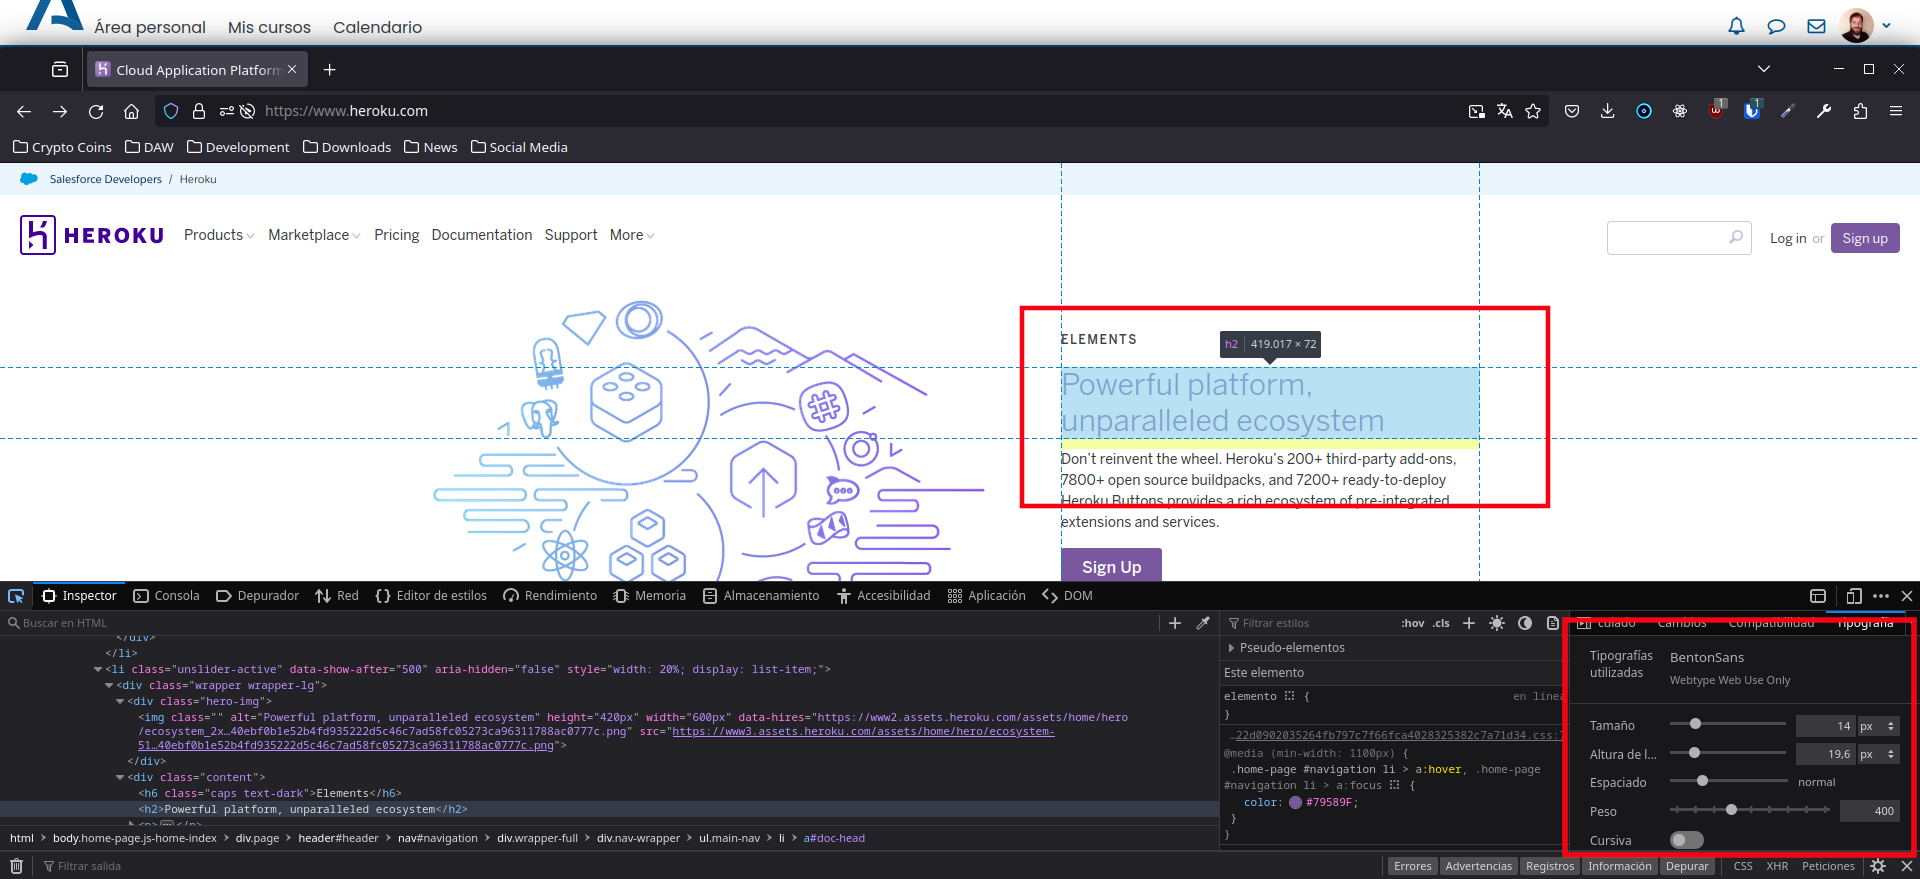
\includegraphics[scale=0.26]{heroku-font.png}
        \end{figure}

        \item  Por último en este ejercicio, vamos a analizar la \textbf{paleta de colores} empleada en la web de Heroku, seleccionando 2 de ellos y explicando donde se usan y cuál es su finalidad.
        \begin{itemize}
            \item \textbf{Púrpura}: este color se usa en los \textbf{botones} de la página, así como en los títulos del contenido y en algunos iconos. Su código de color en \textbf{RGB} es \textbf{\textit{121, 88, 159}} y en hexadecimal es \textbf{\textit{\#79589F}}.

            Según la psicología del color, en este contexto, podemos decir que es usada para transmitir una sensación de \textbf{creatividad e imaginación}.

            \begin{figure}[H]
                \centering
                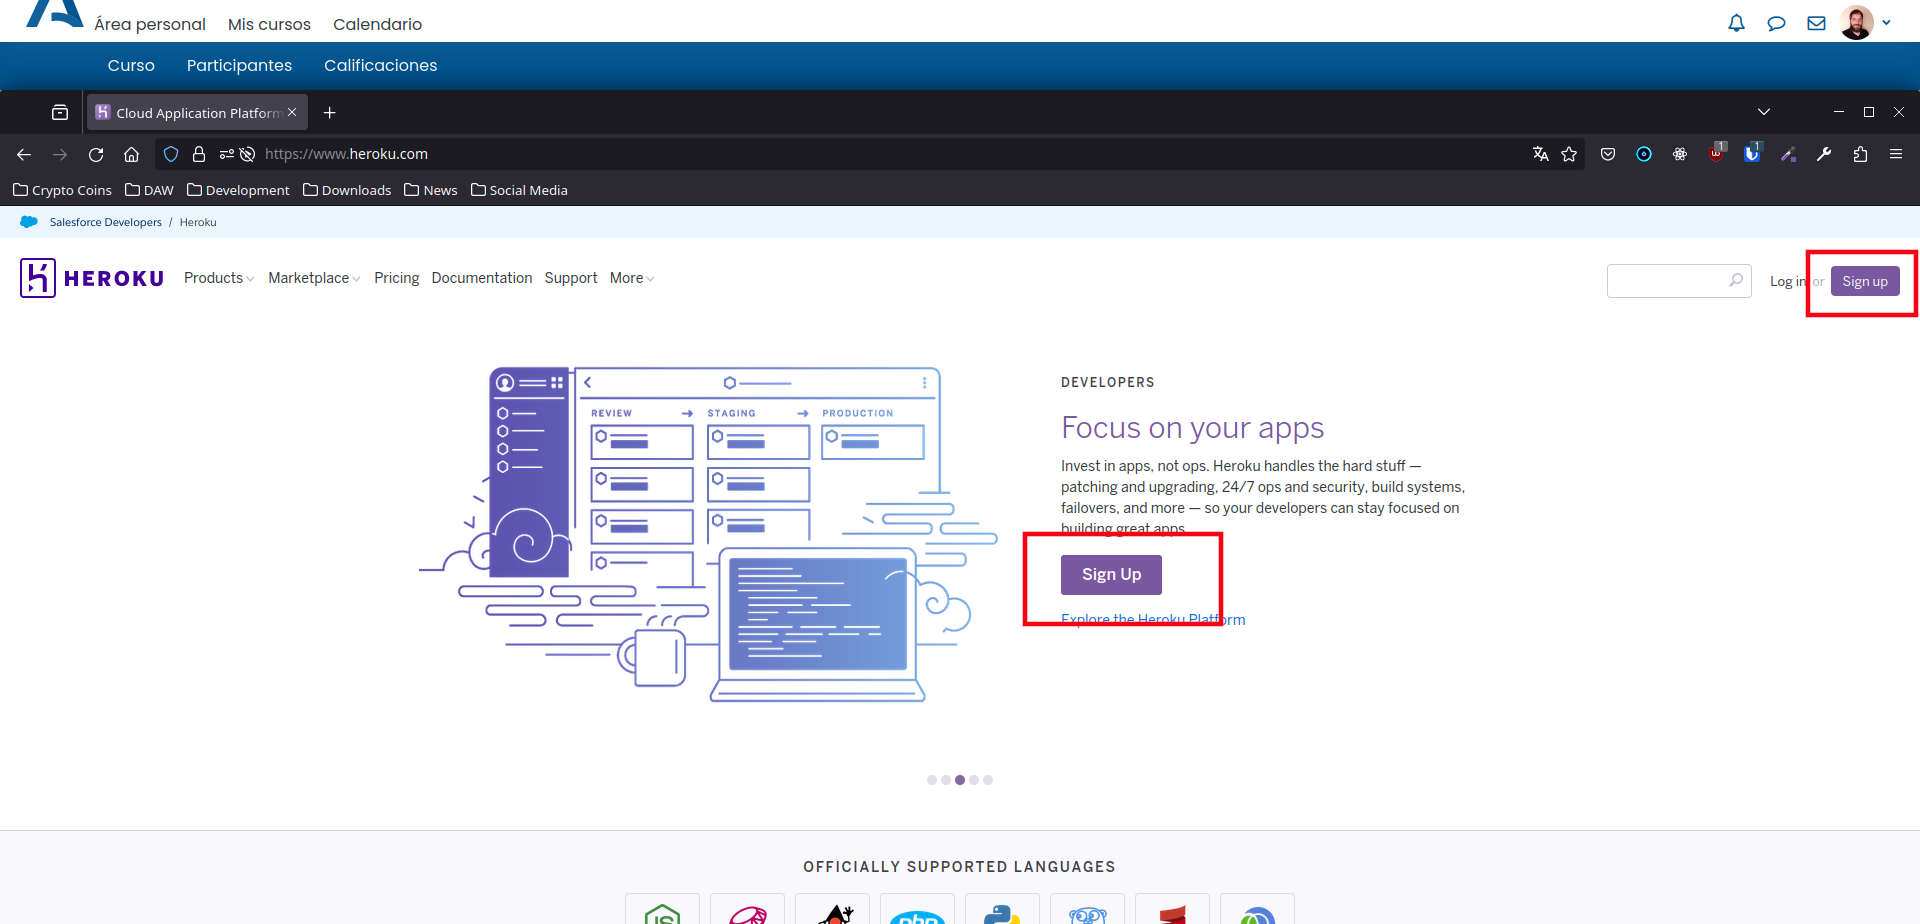
\includegraphics[scale=0.26]{heroku-color-1.png}
            \end{figure}

            \item \textbf{Azul}: se usa especialmente en la parte de contenido dedicada a la empresa Heroku, tanto en el título como en el botón y los iconos que acompañan al texto de esa sección. Su valor RGB es \textbf{\textit{25, 105, 202}} y en hexadecimal \textbf{\textit{1969CA}}.

            En este contexto, y entendiendo que se usa casi exclusivamente en la parte ``más corporativa'' de la web, podemos entender que se usa para transmitir una sensación confianza y seguridad. Es, de hecho, uno de los colores recomendados para diseños corporativos.

            \begin{figure}[H]
                \centering
                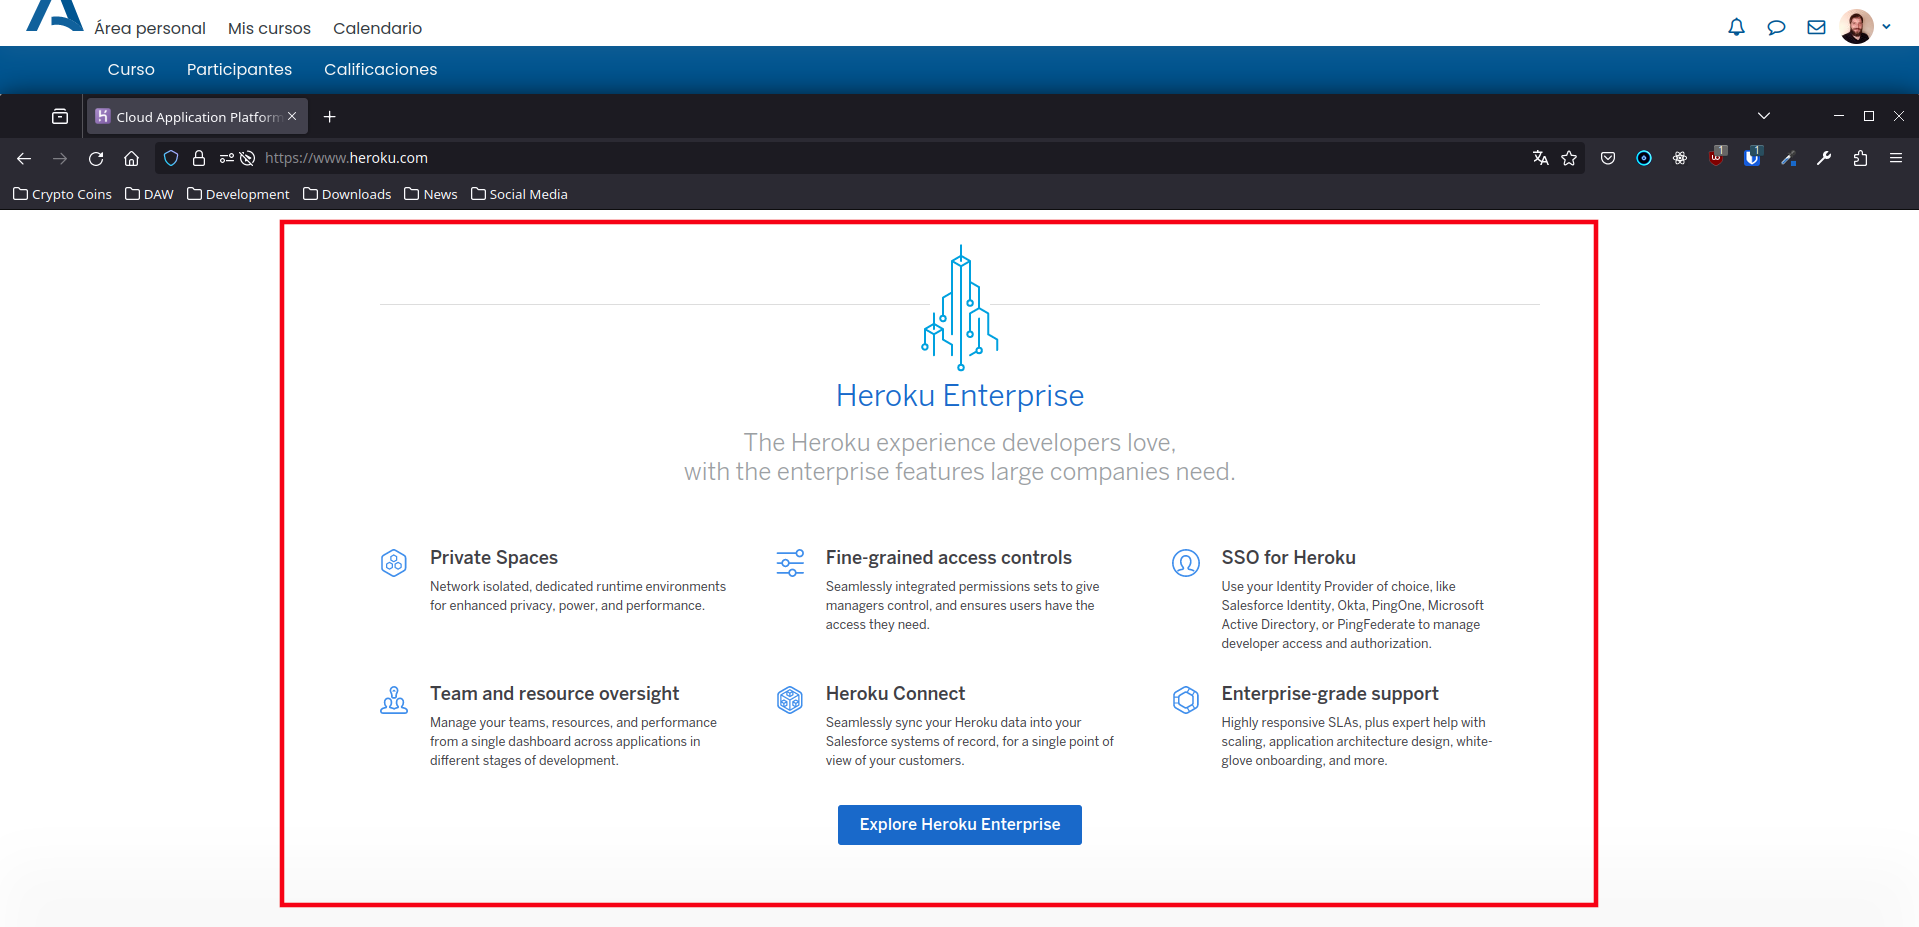
\includegraphics[scale=0.25]{heroku-color-2.png}
            \end{figure}
        \end{itemize}
    \end{itemize}
\end{enumerate}

\section{Ejercicio 5: Boceto Web}
\subsubsection{Enunciado}
Vamos a desarrollar una página Web con una de las temáticas que se han indicado en el inicio de la tarea. Dicha página deberá contener los siguientes bloques:
\begin{itemize}
    \item \textbf{Identificación}: Debe contener un texto (con un color diferente al negro) con tu nombre, apellidos y la foto que aparece en tu perfil de la plataforma.
    \item \textbf{Navegación}.
    \item \textbf{Zona de contenidos}: estará formada por dos zonas y dentro de cada zona habrá al menos una imagen y un texto.
    \item \textbf{Dos zonas de enlaces}: una debe estar encima del pie de página.
    \item \textbf{Pie de página}.
\end{itemize}

Diseña un boceto, utilizando una herramienta digital, donde se vean los diferentes bloques de nuestra Web. Se tendrá en cuenta la claridad del boceto. Añade al fichero de la tarea una captura de pantalla donde se vea el boceto. Por boceto no se entiende el desarrollo HTML5 que tendrás que realizar en el siguiente apartado. Si solo adjuntas el fichero HTML, este apartado no se dará por válido.

\subsection{Solución}
En este ejercicio hemos realizado el boceto de la Web que se nos pide. Para realizar el boceto se ha usado la aplicación \textbf{Figma}.

La web se ha estructurado en 4 zonas diferenciadas:

\begin{itemize}
    \item \textbf{Cabecera}: aquí se ha incluido tanto la foto personal como el nombre y un subtitulo, además de la \textbf{zona de navegación} principal.
    \item \textbf{Cuerpo}: en esta parte se han incluido las \textbf{dos zonas de contenido}. Una con un título, texto, botón e imagen, y otra con un grupo de iconos y sus respectivos textos.
    \item \textbf{Zona de Navegación Inferior}: en esta zona se ha incluido otro menú de navegación.
    \item \textbf{Píe de Página}: en la zona de pie solo se ha incluido información sobre el copyright.
\end{itemize}

El \textbf{color principal} elegido es el \textbf{azul}, para darle un toque corporativo a la web y trasmitir sensaciones de seguridad y confianza. Se han usado diferentes tonos de este color, siendo los códigos hexadecimales de estos colores los siguientes: \textbf{64CCC5}, \textbf{176B87}, \textbf{04364A}  y \textbf{DAFFFB}.

La \textbf{fuente} elegido ha sido \textbf{Roboto}, una fuente \textbf{sans serif} que es bastante cómoda de leer y que además es estéticamente bonita.

En la siguiente imagen, podemos ver el boceto en la herramienta Figma, ya finalizado.

\begin{figure}[H]
    \centering
    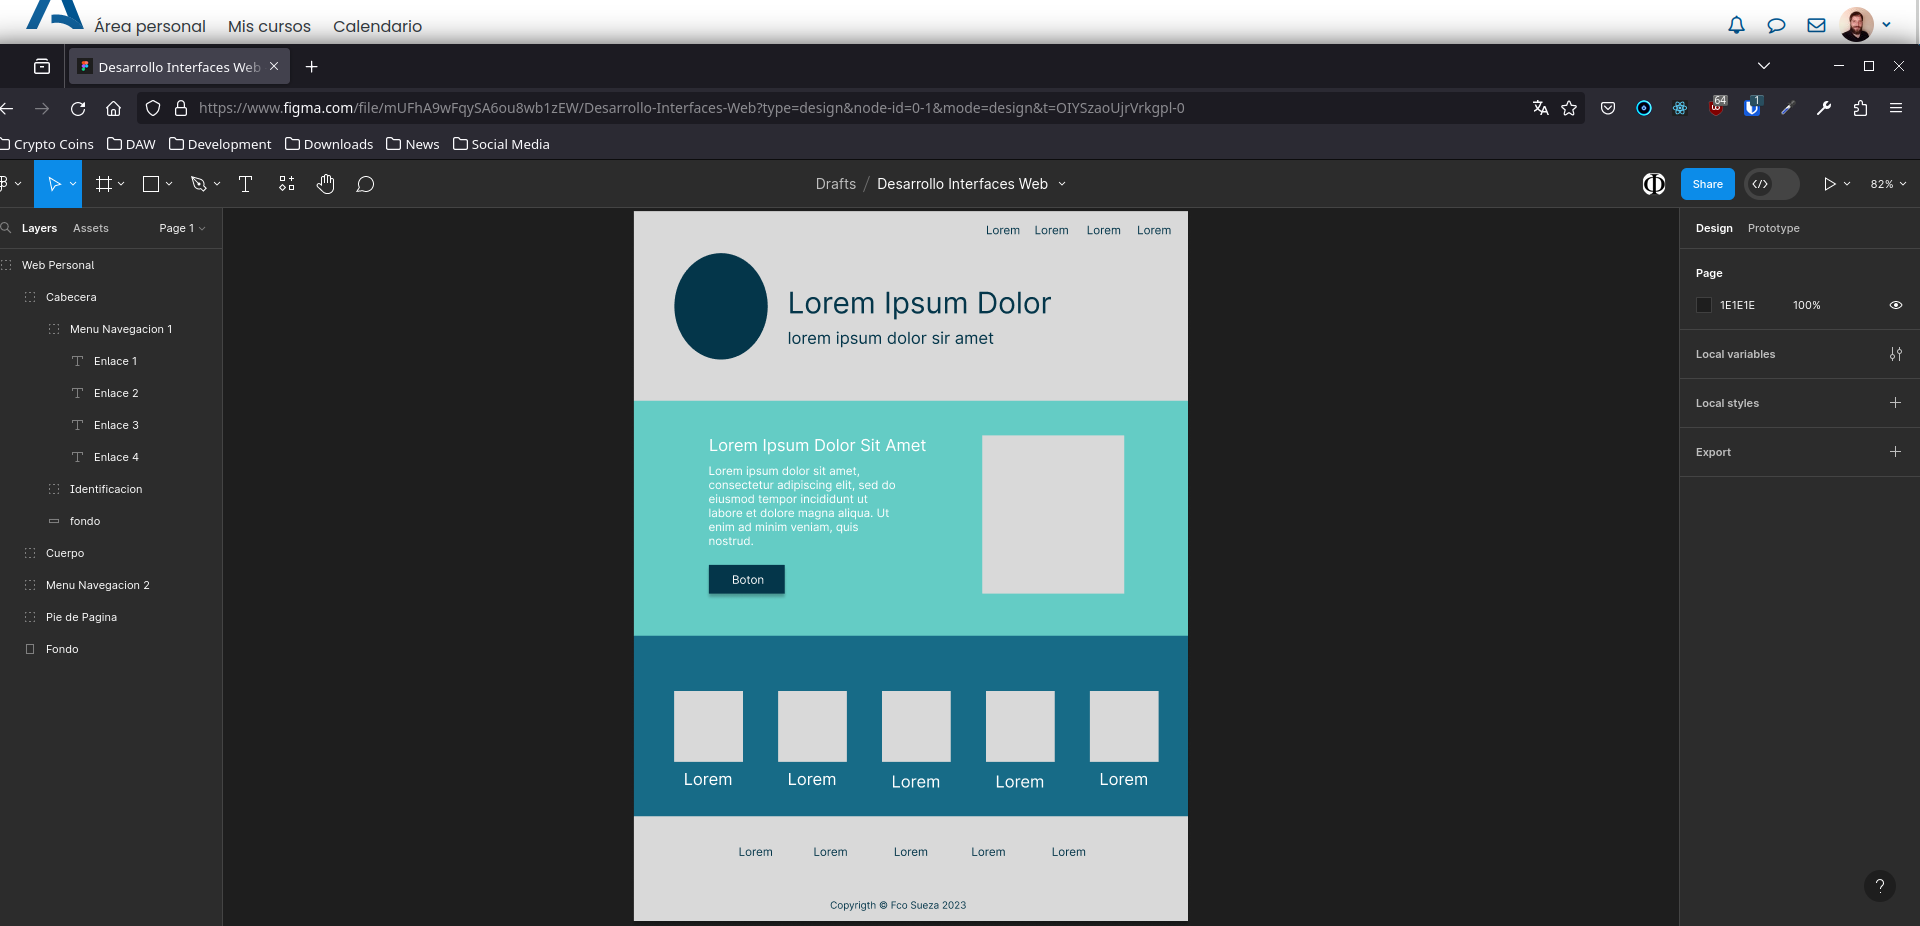
\includegraphics[scale=0.32]{boceto.png}
    \caption{Boceto de la página Web}
\end{figure}

Si se quiere ver más detalladamente el proyecto, se puede consultar este en \href{https://www.figma.com/file/mUFhA9wFqySA6ou8wb1zEW/Desarrollo-Interfaces-Web?type=design&node-id=0%3A1&mode=design&t=Z6PpXOA2wEXOfK2i-1}{la web de Figma}, donde se encuentra alojado.

\section{Ejercicio 6: Desarrollo de la Web}
\subsection{Enunciado}
Desarrolla, usando HTML5 (y CSS si lo crees conveniente y/o necesario), una interfaz donde se vea el diseño realizado en el ejercicio anterior. Para la creación de la página debes utilizar el máximo de etiquetas semánticas. En cada una de las zonas definidas no debe existir ninguna otra información, a excepción de los que se han indicado (cabecera y zona de contenido). Ponle bordes y colores a cada una de las zonas, para que se aprecien de una forma más clara, cada una de las zonas (semánticas) que hay en la página web. Muy importante: no deben utilizarse ni marcos ni tablas, para el posicionamiento de los elementos.

\subsection{Solución}
En este ejercicio se va a implementar la Web de la que hemos realizado el boceto en el ejercicio anterior, para lo que se ha usado HTML y CSS, poniendo especial énfasis en el uso de etiquetas semánticas. Sobre el código cabe anotar:

\begin{itemize}
    \item Para el posicionamiento de los elementos se ha usado \textbf{CSS Flex}.
    \item Se ha seguido la metodología \href{https://getbem.com/introduction/}{BEM} para nombrar las clases CSS.
    \item No se han incluido Media Queries ya que no se pedía en este tema, aunque se han usado \textbf{unidades relativas} para hacer la página un poco más responsiva.
    \item Los diferentes bloques de la web, es decir, identificación, navegación, contenido y píe, han sido marcadas con un \textbf{borde rojo}, aunque este no forma parte del diseño, como se pide en el ejercicio.
    \item Para que la identificación de cada bloque sea mejor, se ha añadido un atributo \textbf{title} a los principales bloques, por lo que si se pasa el ratón por encima del bloque debería mostrar su nombre.
    \item Las ilustraciones utilizadas se han descargado de \href{https://undraw.co/illustrations}{Undraw}.
\end{itemize}

A continuación se muestra una captura de pantalla con parte del resultado final de la web creada. El código se incluirá en el proyecto a entregar.

\begin{figure}[H]
    \centering
    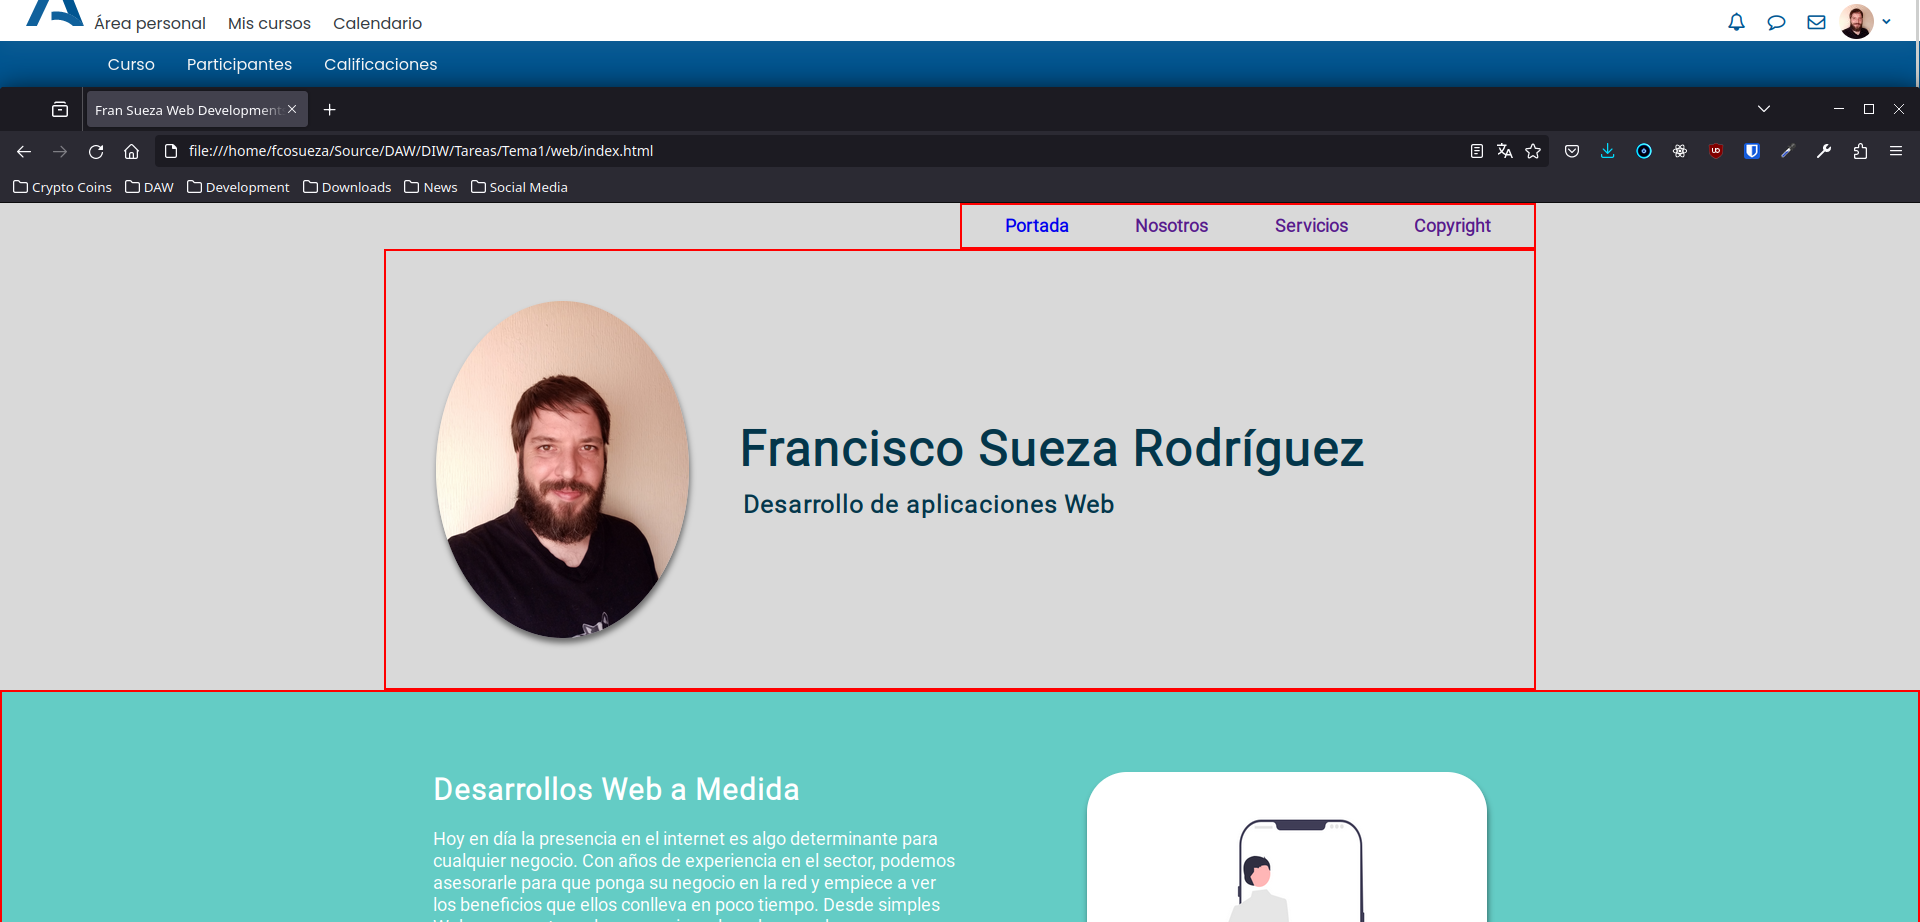
\includegraphics[scale=0.30]{web.png}
\end{figure}

\section{Ejercicio 7: Plantillas Web}
\subsection{Enunciado}
En internet existen multitud de páginas que nos permiten descargar una plantilla y evitar tener que desarrollar una página desde cero. Busca una Web desde donde puedas descargar una plantilla que pueda ser utiliz para nuestro modelo de negocio (indicado al inicio de la tarea), no valdrá un servicio web donde se puedan utiliza plantillas directamente en la web (como por ejemplo IONOS), es decir, tiene que ser una plantilla que pueda descargarse de forma local en tu equipo. Descarga los ficheros de forma local a tu equipo y con esa información realiza lo siguiente:

\begin{itemize}
    \item Indica 2 ventajas y 2 desventajas de utilizar plantillas.
    \item Indica la url de donde has descargado la plantilla. Desde dicha URL debe poderse descargar los ficheros base. Si se pone una URL que no acceda directamente a la plantilla, este apartado no se dará por válido.
    \item Indica los derechos de uso de dicha plantilla. Adjunta captura de pantalla donde se vean claramente los derechos de uso, para justificar la respuesta. Muestra la URL donde se puedan ver dichos derechos de uso.
    \item Sobre la plantilla que has seleccionado tienes que realizar las siguiente acciones, adjuntando las capturas de pantalla que se pidan:
    \begin{itemize}
        \item Mostrar en el navegador la visualización de la plantilla seleccionada sin ninguna modificación donde se vea tu foto de perfil de la plataforma.
        \item Sobre la plantilla base realiza las siguientes modificaciones:
        \begin{itemize}
            \item Cambia el logotipo de la empresa, un icono  o una imagen de la web (solo una modificación, la que prefieras).
            \item Inserta o cambia un título (etiqueta h1,h2, etc.) en la web y asígnale un color (diferente al que tiene).
            \item Realiza otra modificación que te sea interesante.
            \item Adjunta captura de pantalla donde se vea el código original en un editor de código, en la captura debe verse tu foto de perfil.
            \item Adjunta captura de pantalla donde se vea el código que has modificado en un editor de código, en las capturas debe verse tu foto de perfil. Las modificaciones no deben realizarse directamente en la web utilizando el modo desarrollador (no es necesario adjuntar todo el código, solo las partes modificadas)
            \item Explica brevemente junto a a la capturas de modificación en que ha consistido el cambio.
            \item Debes adjuntar tantas capturas de pantalla como modificaciones realices.
        \end{itemize}
        \item Mostrar en el navegador la visualización de la plantilla seleccionada con las modificaciones realizadas donde se vea tu foto de perfil de la plataforma.
    \end{itemize}
\end{itemize}

\subsection{Solución}
En este último ejercicio vamos a usar una \textbf{plantilla web} y a realizar diferentes modificaciones, respondiendo a las diferentes preguntas que se nos plantean.

\begin{itemize}
    \item Las plantillas web tiene sus ventajas e inconvenientes. En este punto, vamos a enumerar 2 ventajas y 2 inconvenientes de su uso.
    \begin{itemize}
        \item \textbf{Ventajas}:
        \begin{itemize}
            \item Son \textbf{fáciles de usar}, ya que solo tenemos que descargarlas y la plantilla estará lista para su uso.
            \item Se pueden \textbf{implementar rápidamente}, realizando los cambios que se adaptan a nuestras necesidades, ahorrándonos tiempo y dinero.
        \end{itemize}

        \item \textbf{Inconvenientes}:
        \begin{itemize}
            \item Las webs creadas con plantillas son \textbf{menos originales}, pudiendo haber cientos de páginas muy parecidas, tantas como desarrolladores hayan usado la misma plantilla.
            \item Muchas de las plantillas que se pueden descargar \textbf{no tienen en cuenta} aspecto importantes de una web como pueden ser \textbf{la usabilidad}, \textbf{la accesibilidad} o \textbf{la experiencia de usuario}, sino que se centran solamente en el apartado estético.
        \end{itemize}
    \end{itemize}

    \item La plantilla que se ha usado se ha descargado de la página web \textbf{plantillashtmlgratis.com}, y en \href{https://plantillashtmlgratis.com/todas-las-plantillas/plantilla/plantillas-html-gratuita-para-descargar-koppee/}{este enlace} podemos ver y \textbf{descargar la plantilla}, así como consultar información sobre el tipo de documento o la licencia.

    \item La \textbf{licencia} de todas las plantillas encontradas en esta página están bajo licencia \textbf{GNU/GPL}, \textbf{creative commons} o de \textbf{dominio público}. En \href{https://plantillashtmlgratis.com/derechos-de-autor/}{este enlace} podemos ver la información referente a los derechos de autor de la plantilla utilizada.

    \item A continuación, se muestra una captura de la pantalla de la plantilla sin modificar.

    \begin{figure}[H]
        \centering
        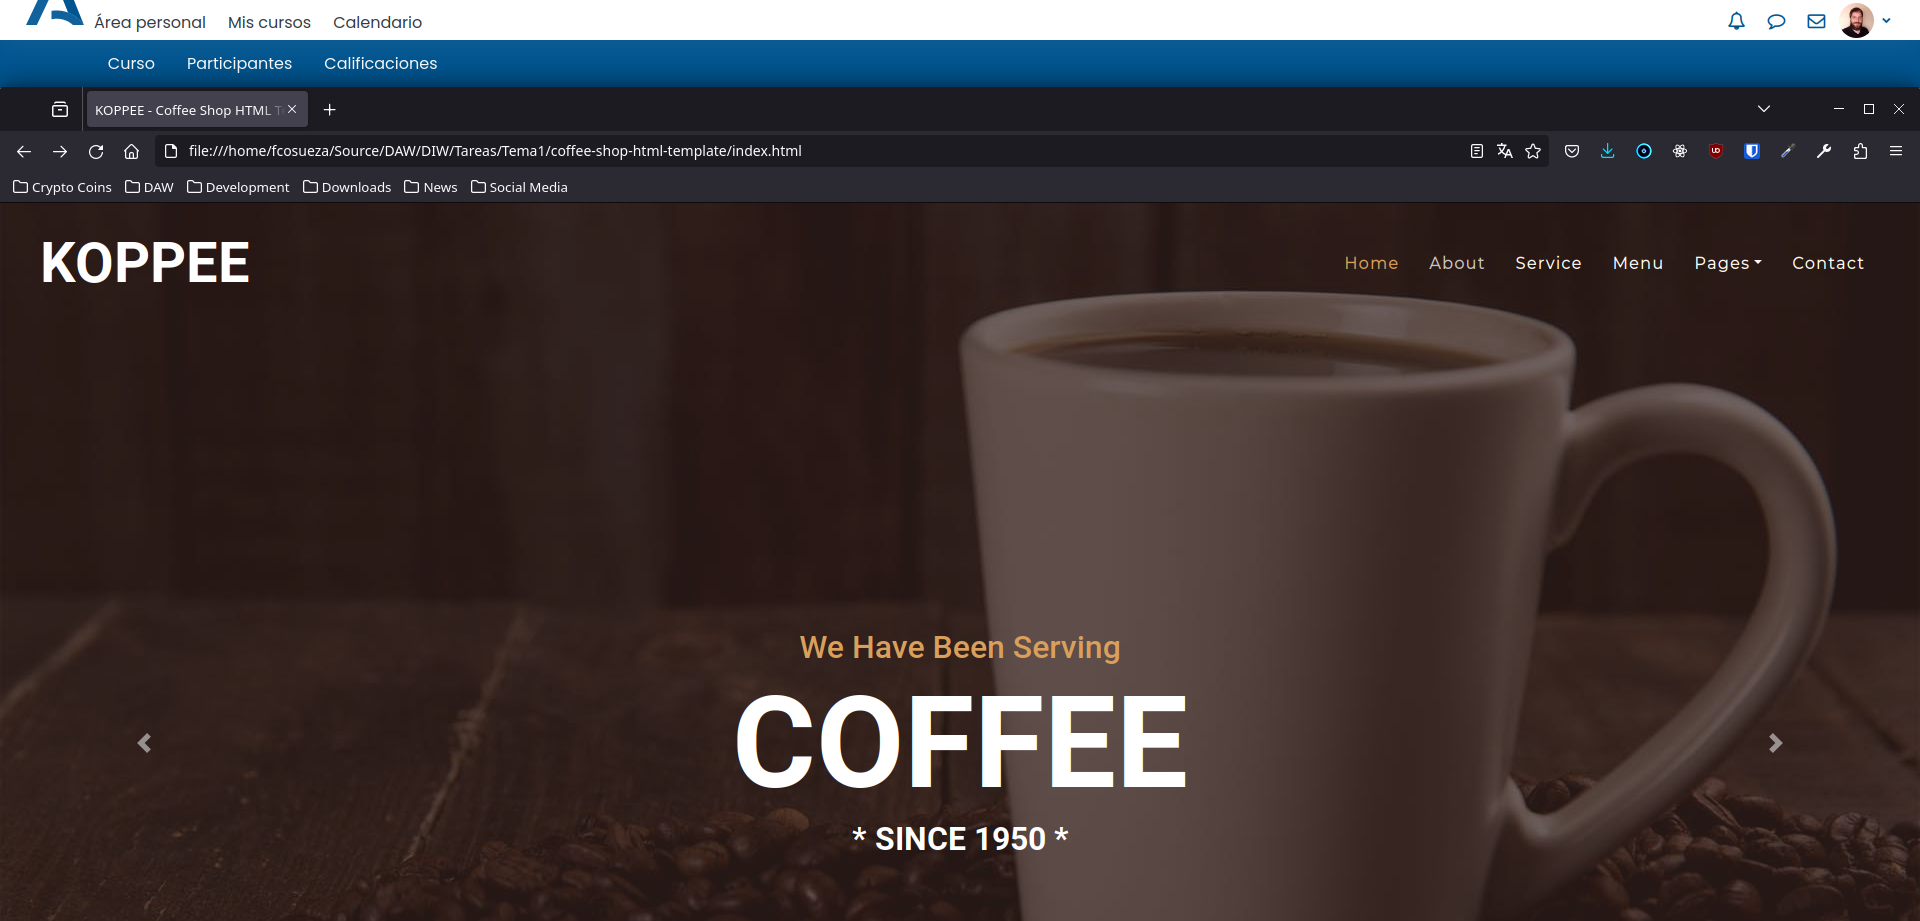
\includegraphics[scale=0.28]{plantilla-original.png}
        \caption{Plantilla descargada sin modificar}
    \end{figure}

    \item En es punto, se van a realizar \textbf{las modificaciones} pedidas sobre la plantilla. Junto con una explicación de la modificación, se mostrará el \textbf{código modificado} en el editor, en este caso, se va a usar VSCode, por lo que no se van a incluir 2 capturas separas, sino que \textbf{se mostrará} el código original y el modificado en \textbf{2 pestañas} del editor, incluyendo una captura del código por cada modificación.

    Todas las \textbf{modificaciones} se van a hacer en la \textbf{página principal de la plantilla}, donde se muestra el carrusel, el menú, etc.., de esta forma, podemos reflejar los cambios realizando una captura similar a la que se ha mostrado con la plantilla sin modificar.

    Las modificaciones estarán resaltadas en el código, ya que se comparará la versión modificad con la original mediante git. De esta forma, se podrá visualizar de forma más rápida el cambio realizado.

    Los \textbf{cambios realizados} han sido los siguientes:

    \begin{enumerate}
        \item En primer lugar se ha modificado la \textbf{primera imagen del carrusel}, hemos elegido otra a nuestro gusto y la hemos incluido en la web. Para llevar esto a cabo, se ha descargado la imagen deseada en la carpeta \textbf{img} proporcionada por la plantilla. Posteriormente, se ha \textbf{modificado el nombre} de la imagen en el código HTML destinado al carrusel.

        Podríamos haber simplemente nombrado nuestra imagen con el mismo nombre que la imagen por defecto y sobreescribirla, pero entonces no habría sido necesario modificar el código HTML, que es le quid de esta actividad. Nuestra imagen la hemos nombrado ``\textbf{hero-1.png}''.

        Una vez descargada, hemos buscado el código HTML en el archivo \textbf{index.html} de la plantilla, el cual está indicado con un comentario, y lo hemos modificado.

            \begin{figure}[H]
            \centering
            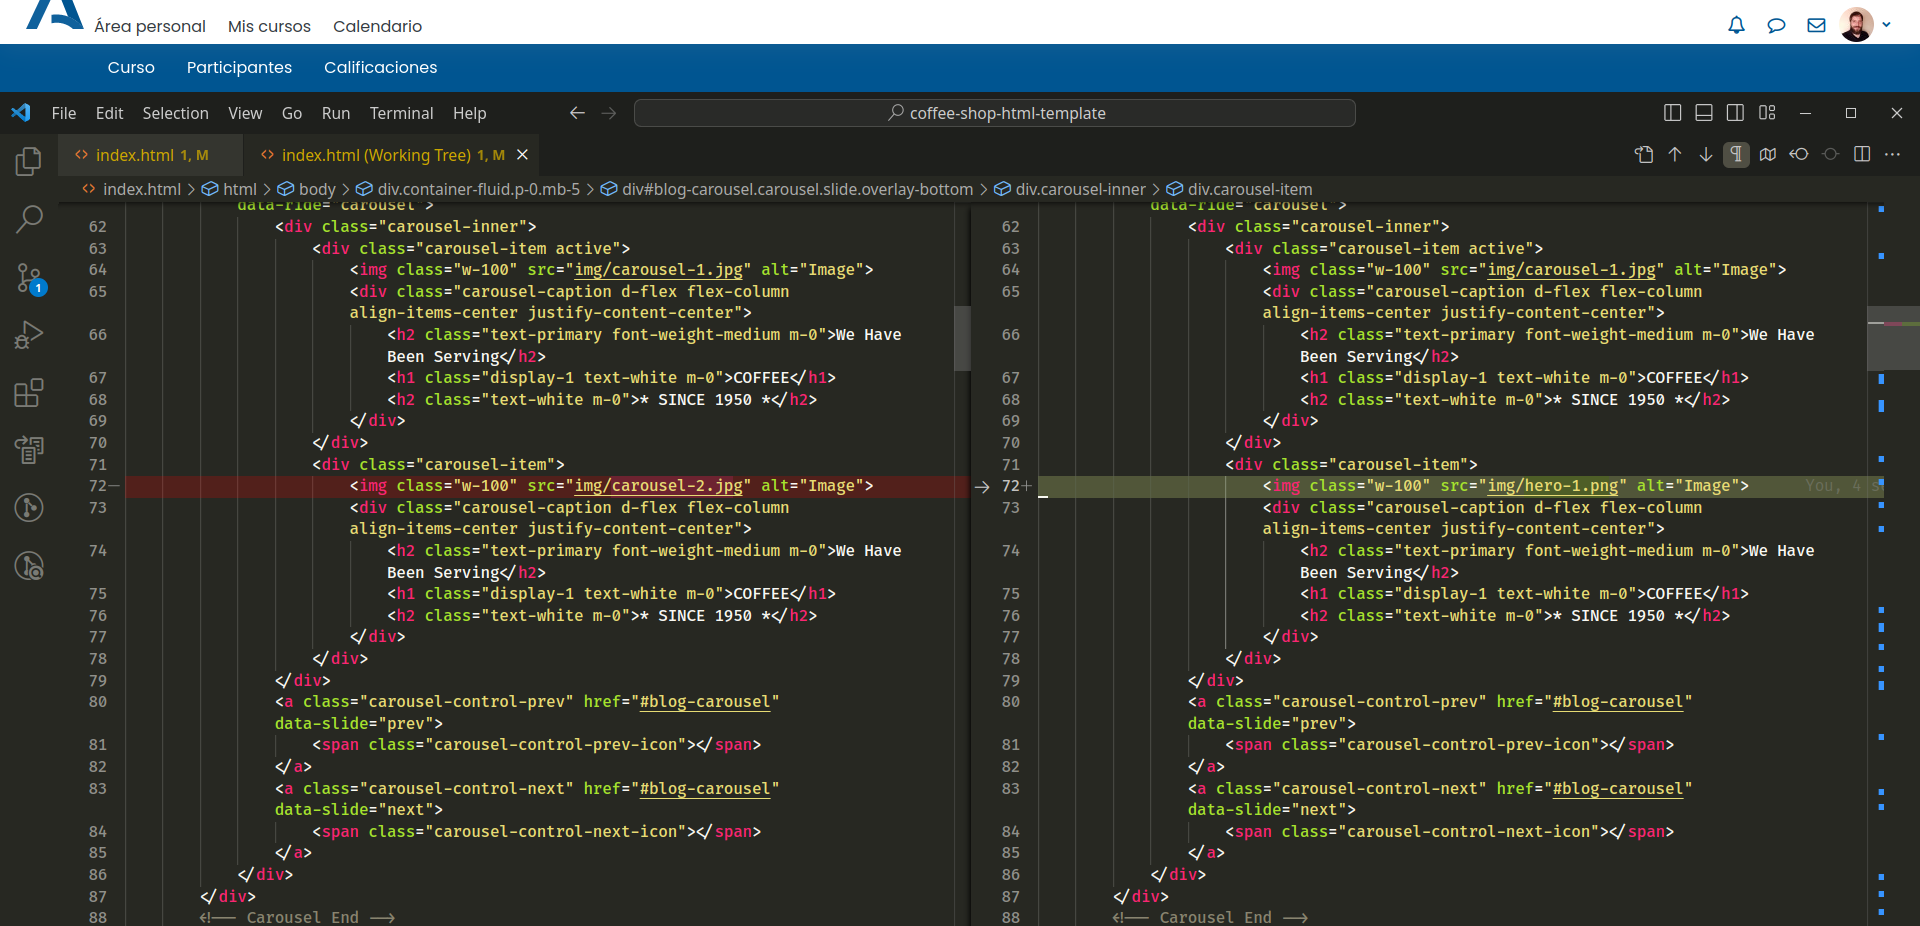
\includegraphics[scale=0.28]{plantilla-cambio-imagen.png}
            \caption{Código HTML sin modificar (izquierda) y modificado (derecha)}
        \end{figure}

        \item El siguiente cambio que se ha realizado ha sido modificar
    \end{enumerate}
\end{itemize}





% Bibliography

%\newpage
%\bibliography{citas}
%\bibliographystyle{unsrt}

\end{document}